\documentclass{article}


% if you need to pass options to natbib, use, e.g.:
\PassOptionsToPackage{numbers, compress}{natbib}
% before loading neurips_2022


% ready for submission
\usepackage{neurips_2022}
\usepackage[utf8]{inputenc} % allow utf-8 input
\usepackage[T1]{fontenc}    % use 8-bit T1 fonts
\usepackage{url}            % simple URL typesetting
\usepackage{nicefrac}       % compact symbols for 1/2, etc.
\usepackage{xcolor}         % colors
\usepackage{booktabs}       % for professional tables
\usepackage{subfigure}
\usepackage{microtype}      % all around better typesetting
\usepackage{amsfonts}
\usepackage{amsthm}
\usepackage{amsmath}
\usepackage{amssymb}
\usepackage{upgreek}
% \usepackage[cm]{fullpage}
\usepackage[colorlinks={true}, citecolor=blue, linkcolor=blue]{hyperref}       % hyperlinks
%\usepackage{algpseudocode}
\usepackage{bbm}
\usepackage{bm}
\usepackage{graphicx}
\graphicspath{{./img/}}
\newtheorem{proposition}{Proposition}
\usepackage{caption}
\usepackage{wrapfig}

% Attempt to make hyperref and algorithmic work together better:
% \newcommand{\theHalgorithm}{\arabic{algorithm}}

% tikz crap
\usepackage{tikz}
\usetikzlibrary{bayesnet}
\usetikzlibrary{arrows}
\usetikzlibrary{backgrounds}



% For theorems and such
\usepackage{mathtools}

% Todonotes is useful during development; simply uncomment the next line
%    and comment out the line below the next line to turn off comments
%\usepackage[disable,textsize=tiny]{todonotes}
\usepackage[textsize=tiny]{todonotes}


% if you use cleveref..
\usepackage[capitalize,noabbrev]{cleveref}


%% \usepackage{array}
%% \usepackage{comment,array,wasysym}
%% \usepackage{graphicx,color,colortbl}

%% % \usepackage{mathptmx} % Use Times as default text font, and provide maths support.  I hate what it does to mathcal so I comment it out
%% % \usepackage{mathtools}
%% % \usepackage{multimedia}
%% % \usepackage{subfigure}
%% %\usepackage{ulem} % for strikethrough \sout
%% \usepackage[normalem]{ulem} % for strikethrough \sout, but avoid the annoying underline in \emph



%% % 
%% % \usepackage[utf8x]{inputenc}
%% % \usepackage{default}

%% % AISTATS sty file doesn't play nicely with caption and subcaption pkgs
%% % \usepackage{caption} 
%% %\usepackage{subcaption}

%% \usepackage{caption}
%% \DeclareCaptionType{copyrightbox}  % Without this, the AISTATs sty creates some clash
%% \usepackage{subcaption}


%% \usepackage{ifthen}
%% \usepackage{enumerate}


%% % 
%% % 
%% %         
%% % \usepackage{yhmath}  % I want really wide tilde. Oren Freifeld, 05/19/2013       




%% %% ICML PACKAGES %%
%% %% \usepackage{ellipsis}

%% %% \usepackage{multirow}

%% %% % Recommended, but optional, packages for figures and better typesetting:
%% %% \usepackage{microtype}
%% %% \usepackage{graphicx}
%% %% % \usepackage{subfigure}
%% %% \usepackage{booktabs} % for professional tables

%% %% % hyperref makes hyperlinks in the resulting PDF.
%% %% % If your build breaks (sometimes temporarily if a hyperlink spans a page)
%% %% % please comment out the following usepackage line and replace
%% %% % \usepackage{icml2018} with \usepackage[nohyperref]{icml2018} above.
%% %% \usepackage{hyperref}

%% %% % Attempt to make hyperref and algorithmic work together better:
%% %% \newcommand{\theHalgorithm}{\arabic{algorithm}}


%%%%%%%%%%%%%%%%%%%%%%%%%%%%%%%%
% COMMENTING MACROS
%%%%%%%%%%%%%%%%%%%%%%%%%%%%%%%%
\newcommand{\RED}[1]{{{\color{red}{#1}}}}
\newcommand{\MAGENTA}[1]{{{\color{magenta}{#1}}}}     
\newcommand{\TODO}[1]{\RED{[TODO: #1]}}
\newcommand{\JLP}[1]{\MAGENTA{[Jason: #1]}}


%%%%%%%%%%%%%%%%%%%%%%%%%%%%%%%%
% THEOREMS
%%%%%%%%%%%%%%%%%%%%%%%%%%%%%%%%
\theoremstyle{plain}
\newtheorem{theorem}{Theorem}[section]
%\newtheorem{proposition}[theorem]{Proposition}
\newtheorem{lemma}[theorem]{Lemma}
\newtheorem{corollary}[theorem]{Corollary}
\theoremstyle{definition}
\newtheorem{definition}[theorem]{Definition}
\newtheorem{assumption}[theorem]{Assumption}
\theoremstyle{remark}
\newtheorem{remark}[theorem]{Remark}

% MI estimators
\newcommand{\Ipost}{\hat{I}_{\text{post}}}
\newcommand{\Imarg}{\hat{I}_{\text{marg}}}
\newcommand{\Iml}{\hat{I}_{\text{m}+p}}

% MRF
\newcommand{\pot}{\psi}
\newcommand{\epmarg}{q}
\newcommand{\logpart}{\Phi}

\def\E{\mathbb{E}}
\DeclareMathOperator*{\argmax}{argmax}
\DeclareMathOperator*{\argmin}{argmin}

% Info Theory Stuff
\newcommand{\KL}[2]{\mathrm{KL}(#1\,\|\,#2)}

%
% List macros
%
\newcommand{\bi}{\begin{itemize}}
\newcommand{\ei}{\end{itemize}}
\newcommand{\deriv}{\mathrm{d}}

\newcommand{\etal}{\textit{et al}}
\newcommand{\FIG}{Fig.~}
%\newcommand{\FIGS}{Figs.~}

 \newcommand{\SEC}{Sec.~}

\newcommand{\eg}{\textit{e.g.}~}
\newcommand{\ie}{\textit{i.e.}~}
\newcommand{\cf}{\textit{c.f.}~}


\newcommand{\EQN}{Eqn.~}
% \newcommand{\EQN}{Equation }
\newcommand{\EQNS}{Eqns.~}
% \newcommand{\EQNS}{Equations }

% distributions
\newcommand{\Dir}{\ensuremath{\text{Dirichlet}}}
 
% integers
\newcommand{\ZZ}{\ensuremath{\mathbb{Z}}}
\newcommand{\RR}{\ensuremath{\mathbb{R}}}
\newcommand{\Rtwo}{\ensuremath{\RR^2}}
\newcommand{\Rthree}{\ensuremath{\RR^3}}
\newcommand{\Rn}{\ensuremath{\RR^n}}
% 
%positive integers
\newcommand{\Zplus}{\ensuremath{\ZZ^+}}
%positive reals
\newcommand{\Rplus}{\ensuremath{\RR^+}}


% n by n matrices
\newcommand{\nBynMats}{\ensuremath{\RR^{n \times n}}}
% m by n matrices
\newcommand{\mBynMats}{\ensuremath{\RR^{m \times n}}}
% n by p matrices
\newcommand{\nBypMats}{\ensuremath{\RR^{n \times p}}}
% 2 by 2
\newcommand{\TwoByTwoMats}{\ensuremath{\RR^{2 \times 2}}}
% 3 by 3
\newcommand{\ThreeByThreeMats}{\ensuremath{\RR^{3 \times 3}}}
% 2 by 3
\newcommand{\TwoByThreeMats}{\ensuremath{\RR^{2 \times 3}}}




% \newcommand{\EqualsDef}{\,{\overset{\text{def}}{=}}\,}
\newcommand{\EqualsDef}{\triangleq}


% set notation
% \newcommand{\set}[1]{\ensuremath{{\left\{#1\right\}}}}
\newcommand{\set}[1]{\ensuremath{{\{#1\}}}}


\newcommand{\InnerProduct}[2]{\left\langle #1,#2 \right\rangle}

\newcommand{\norm}[1]{{{\left\|#1\right\|}}}
\newcommand{\sign}[1]{{\mathrm{sign}\left(#1\right)}}


\newcommand{\ellTwoNorm}[1]{\norm{#1}_{\ellTwo}}


\newcommand{\Acal}{\mathcal{A}}
\newcommand{\Bcal}{\mathcal{B}}
\newcommand{\Ccal}{\mathcal{C}}
\newcommand{\Dcal}{\mathcal{D}}
\newcommand{\Ecal}{\mathcal{E}}
\newcommand{\Fcal}{\mathcal{F}}
\newcommand{\Gcal}{\mathcal{G}}
\newcommand{\Mcal}{\mathcal{M}}
\newcommand{\Ncal}{\mathcal{N}}
\newcommand{\Ocal}{\mathcal{O}}
\newcommand{\Pcal}{\mathcal{P}}
\newcommand{\Qcal}{\mathcal{Q}}
\newcommand{\Tcal}{\mathcal{T}}
\newcommand{\Ucal}{\mathcal{U}}
\newcommand{\Vcal}{\mathcal{V}}
\newcommand{\Wcal}{\mathcal{W}}
\newcommand{\Xcal}{\mathcal{X}}
\newcommand{\Ycal}{\mathcal{Y}}

\newcommand{\MATRIX}[2][cccccccccccccccccccc]{\left[
 \begin{array}{#1}
 #2
 \end{array}
\right]}


\newcommand{\TRACE}{\mathrm{trace}}

\newcommand{\var}[1]{\text{var} \big( #1 \big) }
\newcommand{\cov}[2]{\text{cov} \big( #1,#2 \big)}
\newcommand{\myt}[1]{\widetilde {#1} }

% bold font math 
\bmdefine\balpha{\alpha}
\bmdefine\bbeta{\beta}

\bmdefine\bphi{\phi}


\bmdefine\bb{b}

\bmdefine\bx{x}
\bmdefine\by{y}
\bmdefine\bdotx{\dot{x}}
\bmdefine\bxzero{x_{0}}
\bmdefine\bxone{x_{1}}

\bmdefine\bu{u}

\bmdefine\bv{v}
\bmdefine\br{r}


\bmdefine\bA{A}
\bmdefine\bB{B}

\bmdefine\bS{S}

\bmdefine\bU{U}

\bmdefine\bV{V}
\bmdefine\bX{X}
\bmdefine\bY{Y}


%\bmdefine\balpha{\alpha}

 \newcommand{\Nc}{{N_{c}}}
% \newcommand{\Nc}{N}
\newcommand{\Ne}{{N_{e}}}

% homo coo
\newcommand{\bxh}{\widetilde{\bx}}




\newcommand{\GLn}{\ensuremath{\mathrm{GL(n)}}}
\newcommand{\gln}{\ensuremath{\mathfrak{gl(n)}}}

\newcommand{\GLone}{\ensuremath{\mathrm{GL(1)}}}
\newcommand{\GLtwo}{\ensuremath{\mathrm{GL(2)}}}
\newcommand{\glTwo}{\ensuremath{\mathfrak{gl}(2)}}


% CPA Stuff

\newcommand{\Ac}[1]{A_{c(#1)}}
\newcommand{\Bc}[1]{B_{c(#1)}}

\newcommand{\Vaff}{\Vcal_{\mathrm{aff}}}

\newcommand{\Vpa}{\Vcal_{\mathrm{PA}}}
\newcommand{\Vcpa}{\Vcal_{\mathrm{CPA}}}


\newcommand{\Faff}{\Fcal_{\mathrm{aff}}}

\newcommand{\Fpa}{\Fcal_{\mathrm{PA}}}
\newcommand{\Fcpa}{\Fcal_{\mathrm{CPA}}}

\newcommand{\NSTEPS}{N_{\mathrm{STEPS}}}
\newcommand{\nsteps}{n_{\mathrm{steps}}}


\newcommand{\SigmaPA}{\Sigma_{\mathrm{PA}}}

\newcommand{\SigmaCPA}{\Sigma_{\mathrm{CPA}}}



\newcommand{\Vat}[1]{\bv{(#1)}}
\newcommand{\VatX}{\Vat{\bx}}
\newcommand{\Tat}[2]{T{(#1,#2)}}
\newcommand{\Tinvat}[2]{T^{-1}{(#1,#2)}}
\newcommand{\VatT}[1][t]{\Vat{\Tat{\bx}{#1}}}
% \newcommand{\VatT}[1][t]{\Vat{\Tat{\bx,#1}}}
\newcommand{\VatTinv}[1][t]{\Vat{\Tinvat{\bx}{#1}}}


\newcommand{\IntVatTofX}[1][t]{\int_{0}^{#1}\VatT[\tau]\, d\tau}

\newcommand{\AtimesX}{A{\bxh}}
 

\newcommand{\CpaVatX}{\Ac{\bx}\bxh}
% \newcommand{\CpaVatT}[1][t]{\Ac{\Tat{\bx}{#1}}\widetilde{T}(\bx,#1)}
\newcommand{\CpaVatT}[1][t]{\Ac{\Tat{\bx}{#1}}\widetilde{\Tat{\bx}{#1}}}

\newcommand{\IntCpaVatT}[1][t]{\int_{0}^{#1} \CpaVatT[\tau] \, d\tau}


 

\newcommand{\IntCpaVatTinv}[1][t]{\int_{0}^{#1}  \Ac{\Tinvat{\by}{#1}}\widetilde{\Tinvat{\by}{#1}} \, d\tau}


\newcommand{\CpaVatXasLinComb}{\sum_{j=1}^{d}\alpha_k\Bc{\bx}^{j}\bxh}
\newcommand{\CpaVatTasLinComb}[1][t]{\sum_{j}^{d}\alpha_j\Bc{\Tat{\bx}{#1}}^{j}\widetilde{\Tat{\bx}{#1}}}


\newcommand{\IntCpaVatTLinComb}[1][t]{\int_{0}^{#1}  \CpaVatTasLinComb[\tau] \, d\tau}


% USAGE:
% $\Vat{\bx}$
% $\VatX$
% $\Tat{\bx}{t}$
% $\VatT$
% $\VatT[\tau]$
% $\VatTinv[\tau]$
% $\IntVatTofX$
% $\AtimesX$
% $\Ac{\bx}$
% $\CpaVatX$
% $\IntCpaVatT$
% $\CpaVatXasLinComb$
% $\IntCpaVatTLinComb$



%\newcommand{\VEE}[1]{{#1}^{\vee}}
\newcommand{\VEE}[1]{\mathrm{vec}({#1})}

\newcommand{\HAT}[1]{{#1}^{\wedge}}

 \newcommand{\LCONSTRAINTS}{L_{\mathrm{constraints}}}

% Graph stuff
\newcommand{\parent}{\text{Pa}}
\newcommand{\interventions}{\mathcal{I}}
\newcommand{\alldata}{\mathcal{X}}

% Planning stuff
\newcommand{\actionset}{\mathcal{A}}


% to compile a preprint version, e.g., for submission to arXiv, add add the
% [preprint] option:
%     \usepackage[preprint]{neurips_2022}


% to compile a camera-ready version, add the [final] option, e.g.:
%     \usepackage[final]{neurips_2022}


% to avoid loading the natbib package, add option nonatbib:
%    \usepackage[nonatbib]{neurips_2022}




\title{Fast Variational Estimation of Mutual Information for Implicit and Explicit Likelihood Models}


% The \author macro works with any number of authors. There are two commands
% used to separate the names and addresses of multiple authors: \And and \AND.
%
% Using \And between authors leaves it to LaTeX to determine where to break the
% lines. Using \AND forces a line break at that point. So, if LaTeX puts 3 of 4
% authors names on the first line, and the last on the second line, try using
% \AND instead of \And before the third author name.


\author{%
  Caleb Dahlke \\
  Department of Applied Math\\
  University of Arizona\\
  Tucson, USA \\
  \texttt{calebdahlke@math.arizona.edu} \\
  % examples of more authors
  \And
  Sue Zheng\\
  Analog Devices \\
  Cambridge, MA \\
  \texttt{szheng@csail.mit.edu} \\
  \AND
  Jason Pacheco \\
  Department of Computer Science \\
  University of Arizona\\
  ATucson, USA \\
  \texttt{pachecoj@cs.arizona.edu} \\
  % \And
  % Coauthor \\
  % Affiliation \\
  % Address \\
  % \texttt{email} \\
  % \And
  % Coauthor \\
  % Affiliation \\
  % Address \\
  % \texttt{email} \\
}


\begin{document}


\maketitle


\begin{abstract}
  Computing the mutual information (MI) between sets of random
  variables lacks a closed-form solution in nontrivial
  models. Variational MI approximations are widely used as flexible
  estimators for this purpose, but computing these estimators
  typically requires solving a costly non-convex optimization.  In
  this paper we demonstrate a class of variational estimators whose
  solution is not only convex, but efficiently solved via moment
  matching conditions.  We show that the moment-matched variational
  estimator provides optimal upper and lower bounds on MI in models
  with explicit forward models.  Furthermore, we show that the same
  moment matching solution yields accurate MI approximations in
  so-called "implicit likelihood models", where the observation
  likelihood lacks an analytic representation.  In further analysis on
  implicit likelihood models we prove that our moment matching
  solution is equivalent to existing gradient based methods but at a
  significantly reduced computational cost. Our theoretical results
  are supported by numerical evaluation, showing that the proposed
  approach elegantly applies to fully parameterized (explicit
  likelihood) Gaussian mixture models, as well as implicit models
  arising from marginalization of nuisance variables.  Finally, using
  the SIR model in epidemiology, we show that our approach easily
  applies to implicit simulation-based likelihood models, while
  avoiding costly Likelihood-Free Inference Ratio Estimation (LFIRE)
  common to such models.
\end{abstract}

%% OLD ABSTRACT %%
%% \begin{abstract}
%% Computing the mutual information (MI) between sets of random variables
%% lacks a closed-form in nontrivial models.  Variational approximations
%% provide an efficient mechanism for estimating MI in complex models.
%% However, the presence of nuisance variables results in an implicit
%% relationship between the variables of interest, thus prohibiting the
%% use of most variational MI approximations.  This so-called "implicit
%% likelihood" model is supported by specialized variational
%% approximations, but they can be impractical in realistic settings
%% since they require expensive gradient-based updates.  In this paper we
%% show loose conditions whereby variational approximations over implicit
%% likelihood models can be efficiently solved by simple moment matching
%% operations, thus avoiding the need for costly gradient optimization.
%% Moreover, we prove that moment matching finds the identical solution
%% to existing optimization methods at a significantly reduced
%% computational cost.  We also provide conditions whereby our approach
%% achieves lower approximation error compared to widely used variational
%% MI approximations, even when the likelihood is not implicit.  Our
%% theoretical results are supported by numerical evaluation involving
%% A/B statistical hypothesis testing and nonlinear sensor selection
%% state-space models.
%% \end{abstract}

\section{Introduction}\label{Intro}
%Why we care about MI
In this paper we address a fundamental problem of measuring the
information shared between random quantities.  The focus of this work
is the \emph{mutual information} (MI), which is key in a diverse range
of applications.  For example, in Bayesian optimal experiment design
(BOED)~\cite{lindley56, blackwell50, bernardo79a} MI is used to
measure the amount of information provided by each hypothesized
experiment.  Additionally, MI plays a key roll in measuring and
optimizing the amount of information that can be transmitted along
noisy communication channels~\cite{Cover2006, mackay2003information}.
MI plays a key role in optimizing sensor
configurations~\cite{krause05efficientalgos}, sensor
selection~\cite{WilliamsThesis}, active
learning~\cite{settles2012active}, representation
learning~\cite{tishby2000information}, and many other applications.

% Issues calculating MI
Despite its broad use, exact calculation of MI is typically not
possible.  Sample-based estimates of MI can be inefficient both in
terms of computation and sample complexity.  Such sample-based
estimators require Nested Monte Carlo (NMC) estimation, which exhibits
large finite sample bias that decays slowly~\cite{zheng2018robust,
rainforth2018nesting}. Additionally, straightforward Monte Carlo
estimation cannot be applied in so-called \emph{implicit likelihood}
models that lack a closed-form data generating distribution.  Such
models typically require likelihood-free inference by ration
estimation (LFIRE)~\cite{thomas2022likelihood}, which can be slow due
to repeated fitting of generalized linear models (GLMs) in an
inner-loop~\cite{kleinegesse2021sequential}.

% Variational Methods
Recent variational approaches provide an appealing alternative to MI
estimation by recasting the calculation as an optimization
problem~\cite{poole2019variational}.  Such methods provide convenient
lower bounds~\cite{agakov2004algorithm}, upper bounds, and even apply
in the setting of implicit likelihood models~\cite{Foster2019}.  These
approaches have proven successful in a range of sequential decision
making tasks~\cite{pacheco2019variational, foster2020unified}.  Yet,
despite their computational benefits, computing such estimators can
still be prohibitive due to the underlying non-convex optimization.

%Our Contribution
In this paper we improve the computational properties of several
existing variational bounds and approximations to MI.  We show that
for a class of variational distributions the optimal upper and lower
bounds on MI can be computed by matching moments of the model.  The
resulting estimates are equivalent to existing estimators in previous
work~\cite{poole2019variational, agakov2004algorithm} but we show that
they can be computed with a fraction of the computation.  Furthermore,
we consider the case of MI approximation for implicit likelihood
models.  We show that the same moment matching solution yields
equivalent estimates to existing work~\cite{Foster2019} and minimizes
an upper bound on absolute approximation error.  In doing so we unify
the solution of all three estimators (upper / lower bounds and
implicit approximation) at a fraction of the computational cost of
existing methods.  

%Experiment
We show the accuracy and speed of our approach compared to the
variational and sample-based estimates in a variety of experiments of
both \emph{explicit} and \emph{implicit} likelihood models.  We begin
begin with estimating MI in Gaussian mixtures, for which entropy is
notoriously difficult to compute~\cite{huber2008entropy}.  Our
proposed approach yields accurate estimates with computation that is
capable of scaling to very high-dimensional GMMs.  We then consider
two implicit likelihood models: one, a variation of the generalized
linear model (``Extrapolation Experiment'') from Foster et
al.~(\citeyear{Foster2019}) and the other a simulation-based SIR
Epidemiological model as explored in~\cite{kleinegesse2021sequential}.
In all cases we find that our method offers substantial speedup while
still producing high-quality MI approximations and (when possible) bounds.

%% In this paper, we explore Bayesian inference in the context of
%% decision making.  We specifically explore on the scenario of Bayesian
%% optimal experiment design (BOED)~\cite{lindley56}, where decisions are
%% made to maximize information theortic quantities for a latent variable
%% of interest. Although there are various measures of information,
%% Mutual Information (MI) has been a standard use of information utility
%% (Blackwell, 1950; Bernardo, 1979). It has been used in contexts of
%% sensor planning~\cite{WilliamsThesis}, active learning~\cite{settles2012active} and
%% others.\\


%% %Issues about MI
%% MI faces challenges for many models due to the intracablity of exact MI
%% evaluation. Sample-based estimates of MI can be computationally prohibitive due
%% to the intractibility of the posterior. A na\"ive approach is Nested Monte 
%% Carlo (NMC) approximations which requires many samples to achieve 
%% sufficient accuracy (Rainforth, 2018). Other methods that address the issues of 
%% NMC (Zhang, 2018), sample-based approximations quickly become challenging for 
%% high dimensional latent and observation variables.\\

%% %Previous Methods
%% Alternatives approaches to sample-based estimates include the use of 
%% variational distributions to bound to bound MI. Variational lower 
%% (Barber, 2004) or upper bounds on MI (Foster, 2019) however have no guarantees
%% on the accuracy of their approximation. The bounds are not uniform for each 
%% setting or even each design, therefore bounds can give evaluate decisions
%% higher or lower relative to their true information.\\

%% Other approaches consider reformulating the problem to shift from looking at
%% reducing the uncertainty in the posterior to that estimating the ratio of 
%% the likelihood and marginal. This approach is call likelihood-free
%% infrerence by ratio (LFIRE) (Thomas, 2016).\\

%% %Our Contribution
%% Our approach, considers the use of multiple variational distributions to 
%% approximate the MI. We show the approach lies between the previous variational
%% upper and lower bounds which often results in approximations better than either
%% bound. This approach is also useful in implicit likelihood models as no
%% evalutaions of the model are needed. Furthermore, we show that moment matching 
%% is an efficient optimzaion alternative equivalent to gradient based appraches 
%% for finding optimal variational distributions to both our model as well as the 
%% variational upper and lower bounds.\\

%% %Experiment
%% We show the accuracy of our model compared to the variational bounds and the
%% ground truth in a variety of experiments. We generate a synthetic Gaussian 
%% Mixture Model distribution for comparison of the variational bounds, our
%% method and a ground truth. We also consider an extrapolation model 
%% for comparisons with NMC in the implict likelihood framework. Finally, we 
%% do paramter estimation for the SIR model for comparison with the LFIRE approach.
%% In each approach we highlight the computation speed up given by the moment
%% matching optimization in comparison to the previous gradient based approach.\\


\section{Computing and Approximating MI}\label{background}
Consider an arbitrary joint distribution $p(x,y)$ with latent variable $x$ and
observable variable $y$.  The shared information between these can be
computed via the \emph{mutual information} (MI)~\cite{Cover2006,
mackay2003information}:
\begin{equation}\label{eq:mi}
  I(X;Y) = H(Y) - H(Y \mid X).
\end{equation}
The \emph{marginal entropy} is given by \mbox{$H(Y) = \mathbb{E}[
- \log p(Y) ]$} while the \emph{conditional entropy}
is \mbox{$H(Y \mid X) = \mathbb{E}[ - \log p(Y \mid X) ]$}.  Entropy
expectations are taken with respect to the joint $p(x,y)$.  

\begin{wrapfigure}{r}{0.3\textwidth}
 \vspace*{-10mm}
 \centering
  \tikz{
% nodes
 \node[latent] (z) {$z$};%
 \node[latent,left=of z,fill] (x) {$x$}; %
 \node[latent,right=of z] (y) {$y$}; %
% edges
 \edge {x} {z}
 \edge {z} {y}}
 \caption{\small \textbf{Implicit Likelihood via Nuisance Variables} Likelihood $p(y \mid x)$
 marginalizes  $z$.}
 \label{fig:mc}
\end{wrapfigure}

\subsection{Calculating MI : Explicit and Implicit Models}
Despite its simple definition (\EQN\eqref{eq:mi}) calculating MI is
difficult in practice since entropy terms require exact evaluation of
the probabilities.  For example, calculating the marginal entropy
$H(Y)$ requires evaluation of $\log p(y)$, which often lacks a
closed-form.  Similarly, $\log p(y \mid x)$ may lack a closed-form in
so-called \emph{implicit likelihood models} that require
marginalization of nuisance variables (c.f. \FIG\ref{fig:mc}) or are
defined by simulation as in the SIR model
of \SEC\ref{sec:sir}. Another option is to use the symmetric form
$I(X;Y) = H(X) - H(X\mid Y)$. But this approach requires evaluation of
the posterior $\log p(x \mid y)$, which is also not generally
closed-form.  For these reasons approximations must be considered,
such as the commonly employed sample-based estimators discussed next.
%% Either form may be
%% preferable depending on the dimensions of $X$ 
%% and $Y$ as well as available distributions.  For example, when the
%% dimensionality of observations $Y$ is less than that of $X$ then the
%% form in \EQN\eqref{eq:mi} may be preferred.  However, the marginal
%% entropy $H(Y)$ requires pointwise evaluation of the marginal
%% likelihood $p(y)$, which is typically unavailable.  Furthermore, the
%% posterior $p(x \mid y)$ typically lacks a closed-form.  Finally,
%% so-called \emph{implicit likelihood models} lack explicit
%% representation of the likelihood $p(y\mid x)$, making the calculation
%% of $H(Y \mid X)$ prohibitive.  

\subsection{Nested Monte Carlo (NMC) Estimation}\label{sec:nmc}
%% Despite the seemingly simple definition in \EQN\eqref{eq:mi}, MI
%% typically lacks a closed-form solution.  For example, calculating the
%% marginal entropy $H(Y)$ requires evaluation of the marginal likelihood
%% $p(y) = \int p(x,y) \, dx$, which is not analytic in general.  Similar
%% computational challenges hold for alternate representations.  This
%% motivates the use of approximation, which we briefly discuss.

Given samples $\{(x^i,y^i)\}_{i=1}^N \sim p$ one may use a simple
Monte Carlo procedure to estimate MI,
\begin{equation}\label{eq:nmc}
  \hat{I}_{NMC} = \frac{1}{N} \sum_{i=1}^N \log \frac{ p(y^i \mid x^i)
  }{ \frac{1}{N} \sum_{j=1}^N p(y^i \mid x^j) }
\end{equation}
The use of a plug-in estimator for the marginal
$p(y^i) \approx \frac{1}{N} \sum_j p(y^i \mid x^j)$ makes this a
\emph{nested} Monte Carlo (NMC) estimator.  The NMC is consistent, but
exhibits considerable finite sample bias, as can be shown by Jensen's
inequality~\cite{zheng2018robust, rainforth2018nesting}.  Due to its
bias NMC is often used as a probabilistic bound on MI, but the bound
gap can be significant as bias decays slowly.
%% the plug-in estimate of the marginal likelihood
%% $p(y) \approx \frac{1}{N} \sum_j p(y \mid x^j)$ exhibits significant
%% finite sample bias~\cite{zheng2018robust, rainforth2018nesting}.  
%% This bias can be reduced through different estimation techniques
%% (e.g. leave-one-out), or via robust estimation~\cite{zheng2018robust},
%% but it remains a significant factor.
A bigger limitation is that the NMC estimator (\EQN\eqref{eq:nmc})
requires pointwise evaluation of the conditional probability $p(y \mid
x)$, which may be impossible for simulation-based implicit likelihood
models, such as the SIR Epidemiology model in \SEC\ref{sec:sir}.
%% Consider, for example, the Markov chain
%% in \FIG\ref{fig:mc}.
%% The likelihood is given by
%% \mbox{$p(y \mid x) = \int p(z \mid x) p(y \mid z) \, dz$} which
%% may lack a closed-form.  Such implicit likelihood models will be a
%% core focus of this paper in later sections.


%% This approximation has an error of $KL(p(x|y),q(x|y))$ where $KL$ is
%% the Kullback-Leibler Divergence. This means this is a strict bound
%% except for when $p(x|y)=q(x|y)$ almost surely.\\ The main goal of
%% variational planning is to maximize the bound of \ref{GibbsBound} and
%% then select an action based upon the highest variational mutual
%% information.



%% \subsection{Bayesian Optimal Experimental Design}

%% Let $x$ be a latent variable, $y$ be an observation, and $\mathcal{A}=\{a_1,\dots, a_n\}$ be a set of actions one can take., then the posterior is
%% \begin{equation}
%% p(x|y,a)=p(x)p_a(y|x)
%% \end{equation}
%% Bayesian Optimal Experimental Design aims to find the optimal decision $a^*$ that maximizes information gain
%% \begin{equation}
%% a^* = \argmax_a I_a(X,Y) = H(X)-H_a(X|Y)
%% \end{equation}
%% Where $I_a(X,Y)$ is the Mutual Information of decision $a$ and $H(\cdot)$ is the differential entropy.\\
%% Calculating Mutual Information is not easy as a handful of issues arise. First, the conditional entropy requires evaluations of the posterior, $p(x|y)$, or the predictive prior, $p(y)$, both of which in general may not be found in closed form. 
%% \[H_a(X|Y)=\int p(y)\int p(x|y)\log\dfrac{p(x,y)}{p(y)}dxdy\]
%% A second problem that arises is that the likelihood may be implicit. For a simple example, consider the PGM with three RVs, $x$, $y$ and $z$ as follows

%% \begin{equation}
%% p(y|x)=\int p(z|x)p(y|z)dz
%% \end{equation}
%% In many common and relatively simple cases, the likelihood may not be closed form.\\
%% Due to the difficulties with the distributions, the integral is intractable and standard MC methods cannot be used to evaluate it. A naive approach to circumnavigate this is to try Nested Monet Carlo
%% \begin{equation}
%% I_{NMC}(X,Y) = \dfrac{1}{N}\sum_{n=1}^{N} \log\dfrac{p(y_n|x_{n,0})}{\dfrac{1}{M}\sum_{m=1}^M p(y_n|x_{n,m})}
%% \end{equation}
%% where $x_{n,m}\sim p(x)$ and $y_n\sim p(y|x=x_{n,0})$. However, this has a computation cost of $\mathcal{O}(NM)$ and thus is too computationally expensive in practice.

%% \subsection{Moment Matching}
%% Once a specific member of the Exponential Family, $q(x|\theta)$, has been chosen, the paramters, $\theta$, need to be set. Moment matching is finding the parameters that match the sufficient statistic under expectation from both the target and variational distribution.
%% \begin{equation}
%% \E_{p(x,y)}\left[T(x,y)\right]=\E_{q(x,y|\theta)}\left[T(x,y)\right]
%% \end{equation}
%% Given any target distribution, $p(x|y)$, the member of the Exponential Family, $q(x|y,\theta)$, that minimizes the KL Divergence is the one whose distribution matches moments. So maximizing the bound in \ref{GibbsBound} when restricted to the exponential family amounts to Moment Matching.


\section{Variational MI Estimation}\label{varapprox}
Variational MI estimators~\cite{poole2019variational} address the
computational and sample complexity issues of NMC estimators by
recasting MI calculation as an optimization problem.  In some cases we
can obtain MI bounds using Gibbs' inequality.  The proof is a result
of non-negativity of the Kullback-Leibler divergence, briefly:
$\KL{p}{q} = H_p(q) - H(p) \geq 0$, and so we can bound entropy as
$H_p(q) \geq H(p)$.  In other cases we desire an approximation, rather
than a bound.  We discuss both cases.

\subsection{Variational MI Bounds}
Applying Gibbs' inequality to the conditional entropy $H(X \mid Y)
\leq H_p(q(X \mid Y))$ we have the lower
bound~\cite{agakov2004algorithm},
\begin{equation}\label{eq:mi_post}
  I(X;Y) \geq \max_q \, H(X) - H_p( q(X \mid Y) ) \equiv \Ipost.
\end{equation}
which we call the \emph{variational posterior lower bound}.  Observe
that calculation of the lower bound $\Ipost$ requires evaluation of
the marginal entropy $H(X)$ under the model $p$, which may be
prohibitive.  Applying Gibbs' inequality, instead, to the marginal
entropy $H(X) \leq H_p(q(X))$ we obtain the \emph{variational marginal
  upper bound},
\begin{equation}\label{eq:mi_marg}
  I(X;Y) \leq \min_q \, H_p( q(X) ) - H(X \mid Y) \equiv \Imarg
\end{equation}
Observe that evaluation of the upper bound $\Imarg$ requires
evaluation of the conditional entropy \mbox{$H(X \mid Y)$} under the
model $p$.  For this reason, both bounds ($\Ipost$ and $\Imarg$) apply
only when the model entropy terms can be calculated or
ignored--typically true for sequential decision
making~\cite{pacheco2019variational, Foster2019, foster2020unified,
  agakov2004algorithm}.

\subsection{Variational MI Approximation : Implicit Likelihood Models}
In many cases, the model entropy terms in
\EQNS\eqref{eq:mi_post}~and~\eqref{eq:mi_marg} cannot be calculated 
and so we cannot obtain MI bounds.  By replacing both entropy terms with
their cross-entropies we have the following
approximation~\cite{Foster2019}:
\begin{equation}\label{eq:mi_ml}
  I(X;Y) \approx H_p( q_m(X) ) - H_p( q_p(X \mid Y) ) \equiv \Iml   
\end{equation}
where the variational distributions are $q_m(x)$ (marginal) and
$q_p(x \mid y)$ (posterior).  Reversing the entropy terms yields an
analogous estimator: \mbox{$\hat{I}_{m+\ell} \equiv H_p( q_m(Y) ) -
H_p( q_\ell( Y \mid X ) )$}
%% \begin{equation}\label{eq:mi_implicit}
%%   I(X;Y) &\approx H_p( q_m(Y) ) - H_p( q_\ell( Y \mid X ) ) \equiv \hat{I}_{m+\ell}
%% \end{equation}
Both estimators avoid evaluation of model probabilities, and thus are
useful for implicit likelihood models.  We focus on $\Iml$ for
consistency, but note that our results in \SEC\ref{varoptim} apply
equally to $\hat{I}_{m+\ell}$, which is the form discussed in Foster
et al.~(\citeyear{Foster2019}).  In \SEC\ref{varoptim} we will discuss
how to find the best such approximation.


%% The error of this approximation is the difference of both 
%% cross-entroipy terms errors, that is $KL(p(x)||q(x))-KL(p(x|y)||q(x|y))$.\\


%% NMC has it problem with finite sample bias due to plug-in estimators and has 
%% issues computing implicit likelihoods. Methods have been developed to deal with 
%% these issues or minimze their effect, but ideally, one would like to not have to 
%% deal with them. Variational distributions can be used in this scenario to 
%% "approximate" a denstiy $p(x)$ with a simpler, more computationally tractable 
%% distribution, $q(x)$.

%% \subsection{Variational MI Bounds}
%% With a variational distribution, $q(x)$, we can use the notion of
%% \emph{Cross Entropy}.
%% \begin{equation}
%%   H_p(q(x))=-\int p(x)\log(q(x))dx
%% \label{def:VarEnt}
%% \end{equation}
%% Gibbs' Inequality tells us that cross entropy bounds true entropy, that is
%% \begin{equation}
%%   H_p(p(x))\leq H_p(p(x))+KL(p(x)||q(x))=H_p(q(x))
%% \end{equation}
%% Any distribution we choose to use for the cross entropy term will upper
%% bound the true entropy and the error of the approximation is $KL(p(x)||q(x))$. 
%% Finding an optimal distribution is made easy by simply minimizing the 
%% KL divergence between the true and varitional distribution and equality 
%% holds if and only if $q(x)=p(x)$ almost surely.\\
%% With cross-entropy, for any distribution $q(x)$ we can derive an upper 
%% bound on MI via the \textbf{Variational Marginal Upper Bound}
%% \begin{equation}\label{eq:mi_marg}
%%   I(X;Y) \leq H_p( q(X) ) - H_p(p(x \mid y)) \equiv \Imarg
%% \end{equation}
%% Here, the cross-entropy term bounds the marginal entropy, bounding the 
%% Mutual Infromation from above by and error term of $KL(p(x)|q(x))$.
%% While equation \ref{eq:mi_marg} avoids explicit evaluation of the
%% marginal entropy $H_p(p(x))$, evaluation of the conditional entropy
%% $H_p(p(x \mid y))$ prohibits the use in implicit likelihood models.\\

%% Similarly, using Gibbs' inequality~\cite{agakov2004algorithm} derives 
%% the \textbf{Variational Posterior Lower Bound}
%% \begin{equation}\label{eq:mi_post}
%%   I(X;Y) \geq H(X) - H_p( q(X \mid Y) ) \equiv \Ipost.
%% \end{equation}
%% The cross-entropy terms is used here to bound the conditional 
%% entropy term with a lower bound error of $KL(p(x|y)||q(x|y))$.
%% Calculation of the above bound does not require knowledge of the
%% likelihood, and thus can be used in implicit likelihood settings.
%% However, calculation of the first term $H(X)$ prohibits the use of
%% this estimator in sequential reasoning tasks, since it requires the
%% posterior entropy $H(X \mid \Ycal)$ for some history of observations
%% $\Ycal$.  See~\cite{pacheco2019variational, Foster2019} for more
%% discussion of variational MI bounds in sequential reasoning
%% tasks. Note that both equations \ref{eq:mi_marg} and \ref{eq:mi_post}
%% become tight when $\KL{p}{q} = 0$ almost surely.

%% \subsection{Variational MI Approximation}
%% Because both of the previous bounding methods still require evaluating a
%% true entropy term, $H_p(p(x))$ or $H_p(p(x|y))$, which each give rise to their
%% own problems, Foster et al.~(\citeyear{Foster2019}) propose the
%% following approximation:
%% \begin{equation}\label{eq:mi_ml}
%%   I(X;Y) \approx H_p( q_m(X) ) - H_p( q_p(X \mid Y) ) \equiv \Iml
%% \end{equation}
%% For variational distributions $q_m(x)$ (marginal) and $q_p(x \mid y)$
%% (posterior) the above estimator replaces each of the entropy terms
%% with their cross-entropy $H_p(q)$.  Evaluating this estimator only
%% requires expectations w.r.t. the model, and does not require pointwise
%% evaluation of any model components.  As such, the estimator $\Iml$
%% applies equally well for implicit likelihood models and for sequential
%% decision making.  Note that $\Iml$ is an approximation and is not in
%% general a bound. The error of this approximation is the difference of both 
%% cross-entroipy terms errors, that is $KL(p(x)||q(x))-KL(p(x|y)||q(x|y))$.\\


\section{Moment Matching Variational MI Estimators}\label{varoptim}
%% Variational estimator optimization requires a family of distributions to be 
%% optimized over and a method of optimization. In theory, any family can of 
%% distributions can be chosen but often in partice and in this paper, we will 
%% restrict ourselves to the exponential family for many of its convenient 
%% properties. For optimizing within this family, previous work ~\cite{Foster2019}
%% uses a stochastic gradient approach. We suggest a new technique that is unique
%% to the exponential family which provides significant computation time saves by 
%% avoiding expensive gradient steps.

In general, computing the optimal variational estimators
(e.g. $\Imarg$, $\Ipost$, and $\Iml$) requires solving nonlinear--and
often nonconvex--optimization problems.  In the following sections we
demonstrate a class of variational distributions in the exponential
family that correspond to an efficient convex optimization.
Specifically, for Gaussian variational distributions the optimal
estimators can be solved in closed-form by matching expected
sufficient statistics (means and variances).  The same
(efficient) moment calculation yields optimal (or optimal bounded)
estimators for all three cases.  Unless provided, all proofs can be found in the Appendix.

\subsection{Exponential Families}
Our results rely heavily on properties of the exponential family,
which we briefly review here.  A joint distribution $q(x,y)$ is a
member of the exponential family if the PDF / PMF is of the following
form,
\begin{equation}\label{eq:expfam}
  q(x,y) = h(x,y) \exp \left[\eta^TT(x,y)-A(\eta)\right].
\end{equation}
where $\eta$ are the \emph{natural parameters}, $h(x,y)$ is the \emph{base measure},
$T(x,y)$ the \emph{sufficient statistics}, and $A(\eta)$ is the
\emph{log-partition function}.
The exponential family includes many well-known distributions:
Bernoulli, Categorical, Poisson, Gamma, Gaussian, etc.  In addition to
the natural parameters $\eta$ each exponential family has an alternate
set of \emph{mean parameters} $\mu$, defined as the expected
sufficient statistics: $\mu = \mathbb{E}_q[ T(x,y) ]$. Mean parameters
play a key role in finding projections onto the exponential family, as
shown in Lemma~\ref{lemma:MMKL}.
\begin{lemma}[Moment Matching Projection]\label{lemma:MMKL}
  For any distribution $p(x,y)$ and exponential family $q(x,y)$ whose
  support includes that of $p$ the minimum Kullback-Leibler projection:
  \[
    q^* = \argmin_q \, \KL{p(X,Y)}{q(X,Y)}
  = \argmin_q \, \mathbb{E}_p\left[ \log \frac{p(X,Y)}{q(X,Y)} \right]
  \]
  is convex and the solution given by \emph{moment matching} conditions:
  $\mathbb{E}_p[T(X,Y)] = \mathbb{E}_q[ T(X,Y) ] = \mu^*$
\end{lemma}

%% Then \emph{moment matching} is
%% \begin{equation}\label{eq:mm}
%% \E_{p(x,y)}[T(x,y)]=\E_{q(x,y)}[T(x,y)]
%% \end{equation}
%% If we restrict ourselves to the exponential family, then moment matching minimizes 
%% KL divergence. 

The interested reader can consult the texts~\cite{bishop2006pattern,
murphy2012machine} for a proof of Lemma~\ref{lemma:MMKL} and more
details on the exponential family.  In this paper, we will focus on
Gaussian $q(x,y)$. \FIG\ref{fig:GMMex} shows an example of a GMM,
$p(x,y)$, with a moment matched variational Gaussian, $q(x,y)$ (left),
corresponding marginal projection (center), and resulting variational
estimators (right).
\begin{figure*}[!t]
  \centering \subfigure[Joint pdf
  contour]{ 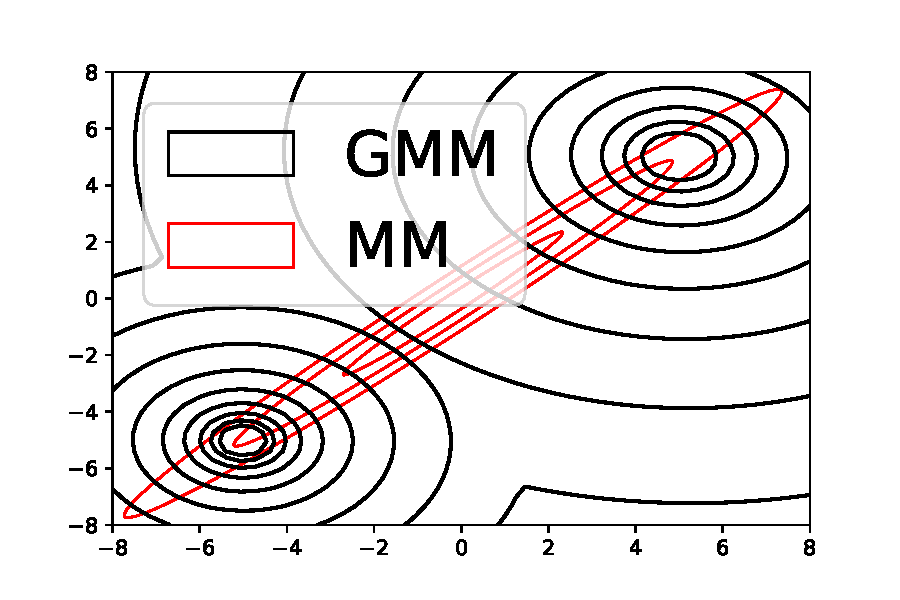
\includegraphics[width=.33\textwidth]{GMMContour.pdf}
  } \subfigure[Marginal
  pdf]{ 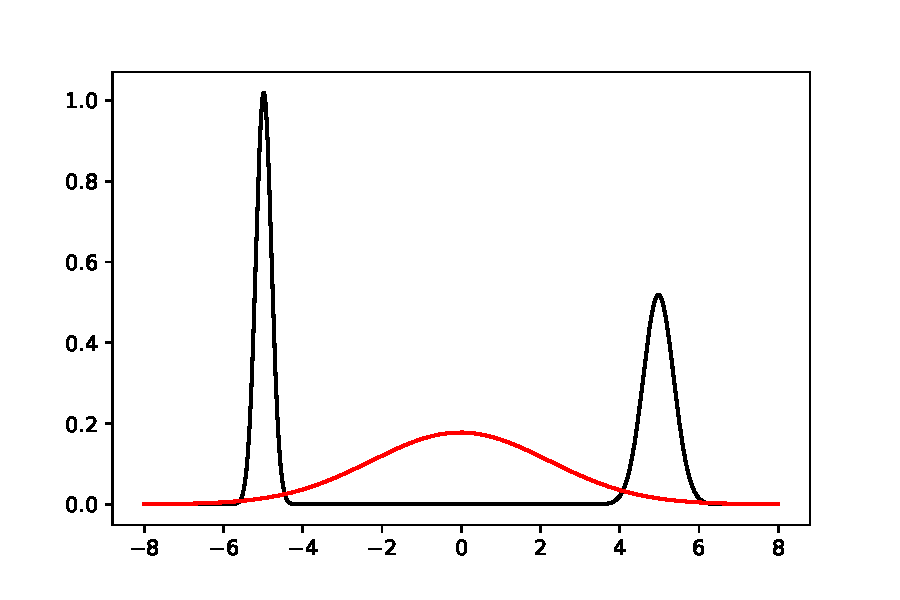
\includegraphics[width=.33\textwidth]{GMMpdf.pdf}
  } \subfigure[MI
  approximations]{ 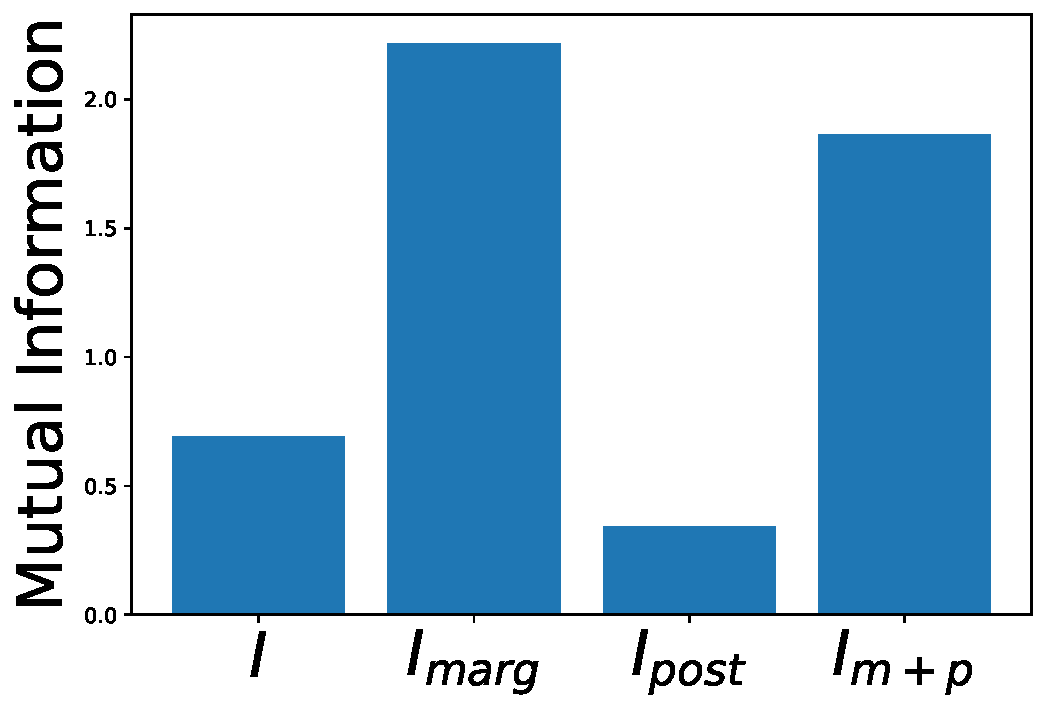
\includegraphics[width=.29\textwidth]{GMMbar.pdf}
  }

  \caption{\small\textbf{Moment Matched Gaussian Mixture Model} (a) A
  bimodal GMM $p$ overlaid with the moment matched Gaussian $q$ has
  its $.5$, $1$, and $1.5$ standard deviation level curves plotted on top in red. (b)
  The marginal PDF is plotted for the Gaussian mixture model and the
  moment matched Gaussian. (c) The true $I(X,Y)$ is shown with
  estimates $\Imarg$, $\Ipost$, and $\Iml$ are all plotted. Notice
  that $\Imarg \geq \Iml \geq \Ipost$.}

  \label{fig:GMMex}
\end{figure*}

%% includes There are many common distributions that fall into this family such as 
%% the Bernoulli distribution, Chi-squared distribution, Wishart distribution, 
%% Gaussian distribution, and many others. Let $q(x,y)$ be in the exponential 
%% family. 

%% The method we propose in this paper matching the moments of a variational 
%% distribution, $q(x,y)$, to those of $p(x,y)$. Our results rely on the properties
%% of the \emph{exponential family}.
%% \begin{definition}{Exponential Family}\\
%%   \emph{
%%   A distribution is a member of the exponential family if it's probability 
%%   density function can be expressed in the form
%%   \[f(x,y|\theta) = h(x,y) \exp \left[\eta(\theta)^TT(x,y)-A(\theta)\right]\]
%%   where $\theta$ are the parameters, $\eta(\theta)$ is the 
%%   natural parameters, $h(x,y)$ is the base measure, $T(x,y)$ is the sufficient 
%%   statistics, and $A(\theta)$ is the log-partition.}
%%   \end{definition}



\subsection{Variational Marginal (upper bound)}\label{sec:varmarg_opt}
To optimize the variational marginal upper bound, $\Imarg$, we must minimze the
bound gap.
\begin{equation}
  I(X;Y) \leq \min_{q_m} \, H_p(q_m(X))-H_p(X \mid Y) = \min_{q_m(X)}H_p(q_m(X)) - \text{const.}
\end{equation}
where the model entropy $H_p(X \mid Y)$ is constant w.r.t. $q_m(x)$
and can be ignored.  If $q_m(x)$ is a Gaussian, then the minimization
is found by moment matching:
\begin{lemma}
  \label{lemma:VMMM} Let $q_m(x)$ be in the exponential family with
  statistics $T(x)$, then for any $p(x,y)$, the optimal $\Imarg^*$ is
  given by moment matching: 
  \[
    \E_{q_m(x)}\left[T(X)\right]=\E_{p(x)}\left[T(X)\right]
  \]  
\end{lemma}
\vspace*{-5mm}\begin{proof} Since $H_p(X)$ is constant in $q_m$ we have,
  \[
    \argmin_{q_m} \, H_p(q_m(X)) = \argmin_{q_m} \,
    H_p(q_m(X))-H_p(X) = \argmin_{q_m} \, \KL{p(X)}{q(Y)}
  \]  
  By Lemma~\ref{lemma:MMKL}, $\E_{q_m(x)}\left[T(X)\right]=\E_{p(x)}\left[T(X)\right]$
  minimizes $\KL{p(X)}{q(Y)}$.
  %% We also know 
  %% $\E_{q(x,y)}\left[T(x,y)\right]=\E_{p(x,y)}\left[T(x,y)\right]$
  %% provides $\E_{q(x)}\left[T(x)\right]=\E_{p(x)}\left[T(x)\right]$.
\end{proof}
Now consider the Gaussian case where $q_m(x)=\Ncal(m,S)$ and a joint
Gaussian $q(x,y)=\Ncal(\mu,\Sigma)$. Moment matching the joint
distribution,
$\E_{q(x,y)}\left[T(X,Y)\right]=\E_{p(x,y)}\left[T(X,Y)\right]$,
provides the marginal moment matching condition. To see this, note
that the marginal moments of the joint are
$q(x)=\Ncal(m_x,\Sigma_{xx})$ where $m_x=m$ is the $x$ component of
the mean and $\Sigma_{xx}=S$ is the block variance of $x$ in $\Sigma$.
Thus, matching the joint Gaussian statistics satisfies
Lemma~\ref{lemma:VMMM} and yields the optimal Gaussian $q_m$ and
corresponding optimal $\Imarg$.



\subsection{Variational Posterior (lower bound)}\label{sec:varpost_opt}
To optimize the variational posterior lower bound, $\Ipost$, we must minimize the
bound gap.
\begin{equation}\label{eq:PostMin}
  I(X;Y) \geq \max_{q_p} \, H_p(X) - H_p(q_p(X \mid Y)) = \min_{q_p} \, H_p(q_p(X \mid Y)) + \text{const}
\end{equation}
The $H_p(X)$ term is constant in $q_p$ and can be ignored for
optimization. The maximization on the left is turned into a
minimization on the right by the negative leading the conditional
entropy.  \EQN\eqref{eq:PostMin} is optimized by satisfying the following
condition,
\begin{lemma}\label{lemma:post_opt}
  If $q_p(x\mid y)$ takes the form of \EQN\ref{eq:ExpFamCond}, then the minimization
  of \EQN\eqref{eq:PostMin} is when
  \begin{equation}\label{eq:OptCrit}
    \E_{p(y)}\left[\E_{q_p(x\mid y)}\left[T(X,Y)\right]\right]=\E_{p(x,y)}\left[T(X,Y)\right]
  \end{equation}
\end{lemma}\vspace*{-2mm}
This result was also shown previously by Pacheco and
Fisher~(\citeyear{pacheco2019variational}).  The condition in
Lemma~\ref{lemma:post_opt} is seemingly a moment matching condition.
However, the l.h.s.~of \EQN\ref{eq:OptCrit} is an expectation
w.r.t.~mixed distributions $p(y)q_p(x\mid y)$, and is difficult to satisfy
in general.  To simplify we consider the joint exponential family
distribution $q(x,y;\eta)$ with natural parameters $\eta$ and
conditional given by,
\begin{equation}\label{eq:ExpFamCond}
  q_p(x\mid y)=q(x\mid y;\eta)=\dfrac{q(x,y;\eta)}{q(y;\eta)}
\end{equation}\label{lemma:OptCrit}
Note that $q(y;\eta)=\int q(x,y;\eta) \, dx$ is not necessarily in the
exponential family.  We can now show that moment matching joint
statistics of $q(x,y;\eta)$ yields the optimal $\Ipost$ via the
following Lemma.
\begin{lemma}\label{lemma:MMOptCrit}
  Let $q_p(x\mid y)$ takes the form of \EQN\ref{eq:ExpFamCond}. Further,
  let the posterior expected statistics be a linear combination of
  marginal statistics as in,\vspace*{-3mm}
  \begin{equation}\label{eq:linearY}
    \E_{q_p(x\mid y)}\left[T(X,Y)\right]=\sum_i^k g_i(\eta)T_{i}(Y)
  \end{equation}
  where $T_i(y)$ is the $i^{th}$ component of the joint statistics
  only depending on  $y$ and $g_i(\eta)$ are arbitrary functions. 
  Then, the optimal $\Ipost$ is given by joint moment matching:
  $\E_{p(x,y)}[ T(X,Y) ] = \E_{q(x,y)}[ T(X,Y) ]$. 
\end{lemma}
Thus both of these conditions imply that moment matching the joint is
optimal for \EQN\eqref{eq:PostMin}. Each of these lemmas are written
in term of an exponential family distribution with some conditions,
since the multivariate Gaussian is the focus of this paper we need to
show that it satisfies these conditions
\begin{corollary}\label{cor:LinearGaussian}
  Let $q(x, y) = \Ncal(m, \Sigma)$ be a Gaussian. Then $q_p(x \mid y)$
  is also Gaussian and satisfies conditions of both
  lemma~\ref{lemma:OptCrit} and lemma~\ref{lemma:MMOptCrit}.
  Furthermore, the optimal $\Ipost$ is obtained by joint Gaussian
  moment matching conditions,\vspace*{-2mm}
  \[
    m^* = \E_{p(x,y)}\left[ (X,Y)^T \right], \qquad \Sigma^* = \text{Cov}_{p(x,y)}\left((X,Y)^T\right)
  \]
  \vspace*{-3mm}And moments of $q_p(x \mid y)$ are the corresponding Gaussian conditional moments
  of $m^*$ and $\Sigma^*$.
\end{corollary}


\subsection{Variational Approximation}\label{sec:varapprox_opt}
Since $\Iml$ is neither an upper nor lower bound, we must minimize the
absolute error
\begin{equation}\label{eq:mi_ml_opt}
  \Iml^* = \argmin_{q_m, q_p} \, \left| I(X;Y) - \Iml(q_m, q_p) \right|
\end{equation}
which is non-convex in general.  We instead minimize the upper bound
as in Foster et al.~(\citeyear{Foster2019}),
\begin{lemma}
  \label{thm:fosterbound} For any model $p(x,y)$ and distributions
  $q_m(x)$, $q_p(x\mid y)$, the following bound holds:
  {\fontsize{9}{10}\selectfont \[\left|\Iml(X,Y)-I(X,Y)\right|\leq
  -\E_{p(x,y)}\left[\log q_m(X)+\log q_p(X\mid Y)\right]+C\]} where
  $C=-H_p(p(X))-H_p(p(X\mid Y))$ does not depend on $q_m$ or
  $q_p$. Further, the RHS is $0$ iff $q_m(x)=p(x)$ and $q_p(x\mid
  y)=p(x\mid y)$ almost surely.  \label{FosterBound2}
\end{lemma}
Previous optimization approaches~\cite{Foster2019} minimize this upper bound using (stochastic) gradient descent:
\begin{equation}\label{eq:sgd_opt}
  q_m^* = \argmax_{q_m} \E_{p(x,y)}[\log(q_m(X))]\hspace{2em}  q_p^* = \argmax_{q_p} \E_{p(x,y)}[\log(q_p(X\mid Y))]
\end{equation}
Note that \EQN\eqref{eq:sgd_opt} does not assume that $q_m(x)$ and
$q_p(x\mid y)$ share a joint distribution $q(x,y)$. We show that under
Gaussianity conditions, not only are optimal $q_m$ and $q_p$ the
marginal and posterior of a joint Gaussian, but that the optimal joint
is found via moment matching.
\begin{theorem}{Equivalence of Moment Matching and Stochastic Gradient Descent}\\
  Let $q_m(x)$ and $q_p(x\mid y)$ be exponential family.  Further, let
  $q_p(x\mid y)$ satisfy the form of \EQN\eqref{eq:ExpFamCond} and the
  linear conditional expectations property (\EQN\eqref{eq:linearY}).
  Then, moment matching the joint distribution $q(x,y)$ yields optimal
  $q_m$ and $q_p$ that minimize the bound on $\Iml$ in
  Lemma \ref{thm:fosterbound}.  \label{EquivMethods}
\end{theorem}
The proof of Theorem~\ref{EquivMethods} (Appendix) follows immediately
from Lemma~\ref{lemma:VMMM} and Lemma~\ref{lemma:MMOptCrit}.
%% says that
%% moment matching the joint minimizes $-\E_{p(x,y)}\left[\log
%% q_m(x)\right]$.  Lemma ~\ref{lemma:OptCrit} and ~\ref{lemma:MMOptCrit}
%% show that moment matching the joint minimizes $-\E_{p(x,y)}\left[\log
%% q_p(x\mid y)\right]$.
Finally, we show that the general result in Theorem
~\ref{EquivMethods} is satisfied for Gaussian $q_m(x)=\Ncal(m,S)$ and
a linear conditional Gaussian $q_p(x\mid y)=\Ncal(Ay+b,\Sigma_p)$
satisfy. 
\begin{corollary}
  Let $q_m(x)=\Ncal(m,S)$ and $q_p(x\mid y)=\Ncal(Ay+b,\Sigma_p)$. Then theorem 
  ~\ref{EquivMethods}  is satsified and thus moment matching a Joint Gaussian 
  $q(x,y)=\Ncal(\mu, \Sigma)$ will minimize lemma~\ref{thm:fosterbound}.
\end{corollary}


\subsection{Properties of Variational Estimators}
We pause here to reflect on the implication of our results
in \SEC\ref{sec:varmarg_opt} - \ref{sec:varapprox_opt}.  Namely, for
joint Gaussian variational $q(x,y)$ all optimality conditions are
satisfied by joint moment matching.  Thus, the same moment-matched
joint Gaussian is optimal for all three variational estimators.  For
the approximation $\Iml$, joint moment matching is equivalent to
optimizing an upper bound on error, but is not globally optimal in
general.  We conclude this section with additional properties of these
estimators.  For example, it is trivial to show that they obey the
following ordering:
%% The $\Imarg$ and $\Ipost$ are often useful because they are bounds. $\Iml$, on 
%% the other hand, is neither an upper bound or lower bound, however this 
%% approximation can be placed between the variational marginal and variational 
%% posterior bounds.\\
\begin{lemma}
  For any $q_m(x)$ and $q_p(x\mid y)$, $\Ipost\leq\Iml\leq\Imarg$.
  \label{lemma:MIOrder}
\end{lemma}
Thus, $\Iml$ is never the least accurate out of all three methods. If
$\Iml$ is an over approximation, it is a tighter upper bound than
$\Imarg$ and the converse holds if it is an under approximation (it is
a tighter than $\Ipost$). We can also ask when $\Iml$ is closer in
absolute error than either of the bounds
\begin{lemma}\label{lemma:AbsPostError}
  For a variational $q_m(x)$ and $q_p(x\mid y)$, if 
  \begin{enumerate}
    \item If $\KL{p(X\mid Y)}{q(X\mid Y)}\geq \frac{1}{2}\KL{p(X)}{q(X)}$ 
    then $\Iml$ has lower error than $\Ipost$
    \item If $\KL{p(X)}{q(X)}\geq \frac{1}{2}\KL{p(X\mid Y)}{q(X\mid Y)}$ 
    then $\Iml$ has lower error than $\Imarg$
  \end{enumerate}
\end{lemma}
While these conditions cannot be checked in practice they do offer
some insight.  For example, if $q_m(x)$ approximates $p(x)$ about as
well as $q_p(x\mid y)$ approximates $p(x\mid y)$ (in KL) then $\Iml$ is the
best approximation to use.

\paragraph{Moment matching stationary point} is not always a local minimum to the 
optimization of $\Iml$. Consider \FIG\ref{fig:MMoptimal} where a two
dimensional Gaussian is moment matched to Gaussian mixture models. All
of the parameters of the moment matched Gaussian are held constant but
the correlation parameter, $\rho$, is varied an the absolute error of
$\Iml$ is plotted. In one case, the minimum is found and any changed
value of $\rho$ results in a worse approximation of MI. However is the
second case, a local maximum is found, and we notice that there is a
range of values for $\rho$ that result in not only better
approximations of MI, but sometimes exact.  Exploring this property is
a topic of future work.

\begin{figure*}[!t]
  \centering
  \subfigure[Local minimum]{
    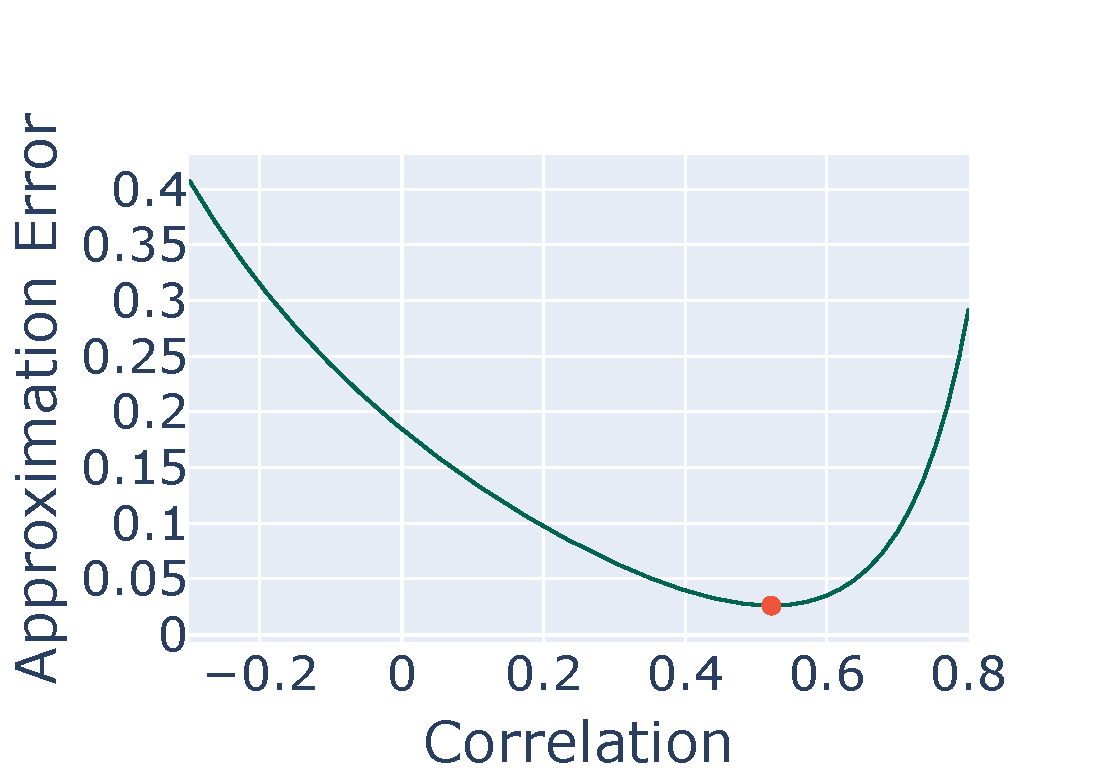
\includegraphics[width=.4\textwidth]{MMMinimum.pdf}
    }
  \subfigure[Local maximum]{
  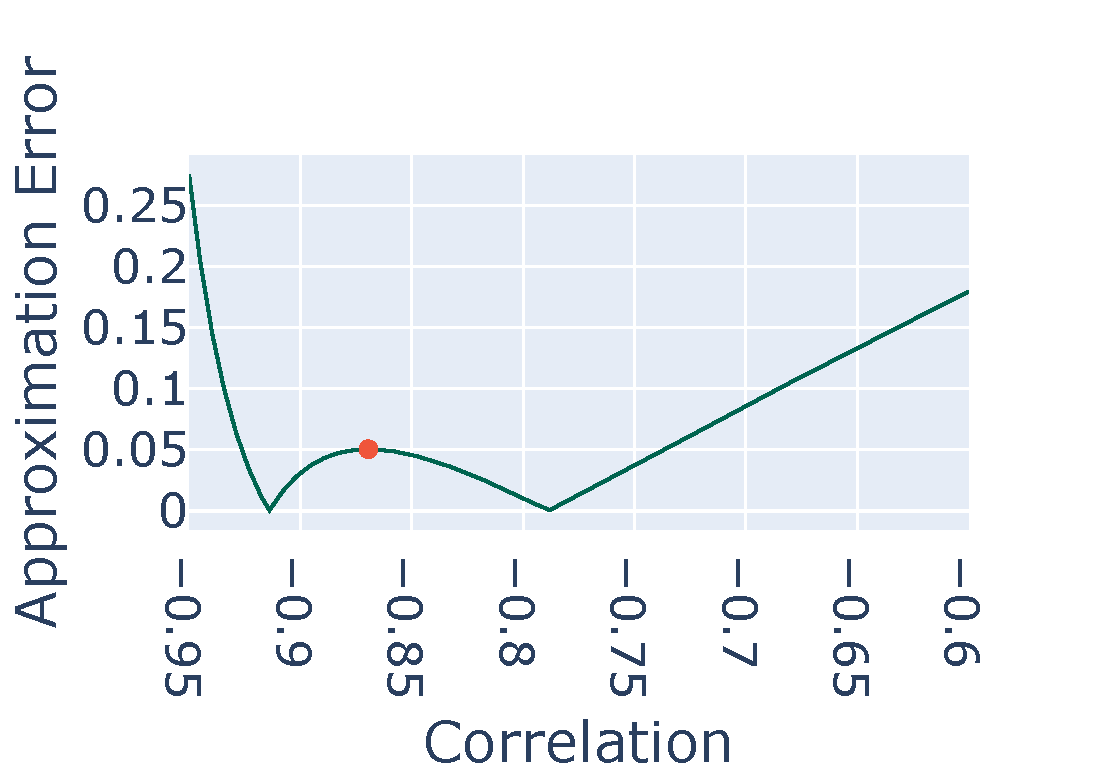
\includegraphics[width=.4\textwidth]{MMMaximum.pdf}
  }
  \caption{\small\textbf{Moment Matched Optimum} (a) The moment matching solution 
  (red) is the local minimum as a variational apprximation to a GMM. (b) For a 
  seperate GMM, the moment matched solution is a local maximum and there is a 
  range of values for $\rho$ that result in better approximation, and two that 
  result in exact values of MI.}
  \label{fig:MMoptimal}
\end{figure*}



% Each variation method has its own error which must be minimized, $\Imarg$ has 
% an error of $KL(p(x)||q(x))$, $\Ipost$ has an error of $KL(p(x|y)||q(x|y))$, 
% and $\Iml$ has an error of $KL(p(x)||q(x))-KL(p(x)||q(x))$. Finding the best 
% approximation $\Iml$ requires minimizing the approximation error,
% \begin{equation}\label{eq:mi_ml_opt}
%   \Iml^* = \argmin_{q_m, q_p} \, \left| I(X;Y) - \Iml(q_m, q_p) \right|
% \end{equation}
% which cannot be computed in general.  Foster et
% al.~(\citeyear{Foster2019}) instead minimize an upper bound provided
% in the following lemma,
% \begin{lemma}
%   \label{thm:fosterbound}  
%   For any model $p(x)p(y|x)$ and distributions $q_m(x)$ and
%   $q_p(x|y)$, the following bound holds:
%   {\fontsize{9}{10}\selectfont
%     \[\left|\widetilde{I}(x,y)-I(x,y)\right|\leq -\E_{p(x,y)}\left[\log q_m(x)+\log q_p(x|y)\right]+C\]}
%   where $C=-H_p(p(x))-H_p(p(x|y))$ does not depend on $q_m$ or
%   $q_p$. Further, the RHS is $0$ iff $q_m(x)=p(x)$ and
%   $q_p(x|y)=p(x|y)$ almost surely.
%   \label{FosterBound2}
% \end{lemma}
% A proof of Lemma~\ref{thm:fosterbound} is reproduced in the appendix. 
% \paragraph{Optimization methods} suggested by previous work ~\cite{Foster2019} is
% \emph{stochastic gradient descent}.
% \begin{equation}\label{eq:sgd_opt}
%   q_m^* = \argmax_{q_m} \E_{p(x,y)}[log(q_m(x))]\hspace{2em}  q_p^* = \argmax_{q_p} \E_{p(x,y)}[log(q_p(x|y))]
% \end{equation}
% Lemma ~\ref{thm:fosterbound} is found by seperately finding $q_m^*$ and $q_p^*$ by 
% equation \ref{eq:sgd_opt}. For $\Imarg$, the optimal distribution is found by 
% just finding $q_m^*$ and the optimal distribution for $\Ipost$ is just $q_p^*$.


% \subsection{Optimizing $\Iml$}
% To minimize the bound in Lemma~\ref{thm:fosterbound}, an optimal 
% marginal, $q_m$ and posterior, $q_p$, must be found.

% \subsubsection{Stochastic Gradient Descent}
% Previous work suggests finding the maximum by separately optimizing a Gaussian 
% marginal $q(x)=q_m(x)$ and Gaussian posterior $q(x|y)=q_p(x|y)$ though stochastic 
% gradient ascent. That is he separately calculates the following:
% \begin{equation}\label{eq:sgd_opt}
%   q_m^* = \argmax_{q_m} \E_{p(x,y)}[log(q_m(x))]\hspace{2em}  q_p^* = \argmax_{q_p} \E_{p(x,y)}[log(q_p(x|y))]
% \end{equation}
% It is important to note that this does not assume that $q_m(x)$ and $q_p(x|y)$ share 
% a joint Gaussian, $q(x,y)$, that they are both derived from. This approach will 
% find our optimal distribution to minimize the bound in Lemma~\ref{thm:fosterbound} 
% however this requires two optimization operations to be computed which can be 
% time consuming, especially with higher dimensional problems.

% \subsubsection{Moment Matching}
% The method proposed in this paper, instead of computing Gradient Descent, we will
% match the moments of $q(x,y)$ to those of $p(x,y)$. To define what this means, 
% we first intrduce the \emph{Exponential Family}
% \begin{definition}{Exponential Family}\\
%   \emph{
%   A distribution is a member of the Exponential Family if it's probability 
%   density function can be expressed in the form
%   \[f(x,y|\theta) = h(x,y) \exp \left[\eta(\theta)^TT(x,y)-A(\theta)\right]\]
%   where $\theta$ are the parameters, $\eta(\theta)$ is the 
%   Natural Parameters, $h(x,y)$ is the base measure, $T(x,y)$ is the sufficient 
%   statistics, and $A(\theta)$ is the Log-partition.}
%   \end{definition}
% There are many common distributions that fall into this family such as 
% the Bernoulli distribution, Chi-squared distribution, Wishart distribution, 
% Gaussian distribution, and many others. The case of the Multivariate Gaussain
% will be the focus of this paper but results can be expanded to include other 
% distributions from the exponential family as well.

% Let $q(x,y)$ be in the Exponential Family. Then \emph{Moment Matching} is
% \begin{equation}
% \E_{p(x,y)}[T(x,y)]=\E_{q(x,y)}[T(x,y)]
% \end{equation}
% and the resulting marginal and likelihood are used as the approximating distributions
% \begin{align}\label{eq:mm_opt}
% q_m^*(x)=q_\eta(x)=\int q_\eta(x,y)dy \hspace{2em} q_p^*(x|y)=q_\eta(x|y)=\dfrac{q_\eta(x,y)}{\int q_\eta(x,y)dx}
% \end{align}
% In this paper, we will focus on the case where $q(x,y)$ is the Multivariate 
% Gaussiian in the exponential family. Figure ~\ref{fig:GMMex} shows an example of 
% a Gaussian Mixture Model, $p(x,y)$, with a moment matched variational Gaussian, 
% $q(x,y)$. Notice that the moment matching finds the mean of the nodes and then 
% matches the varaiance to capture both nodes. This Gaussian is then used as the 
% variational distribution for each of the variational methods and their outputs 
% compared. The ordering of each method matches Lemma ~\ref{lemma:MIOrder}.
% We will show that for Gaussian variational families, the optimal $q_m$ 
% and $q_p$ found in equation \ref{eq:sgd_opt} share a unique optimal joint. 
% We further show that the optimal joint distribution is given by moment matching.
% \begin{figure*}[!htb]
%   \centering
%   \subfigure[Joint pdf contour]{
%   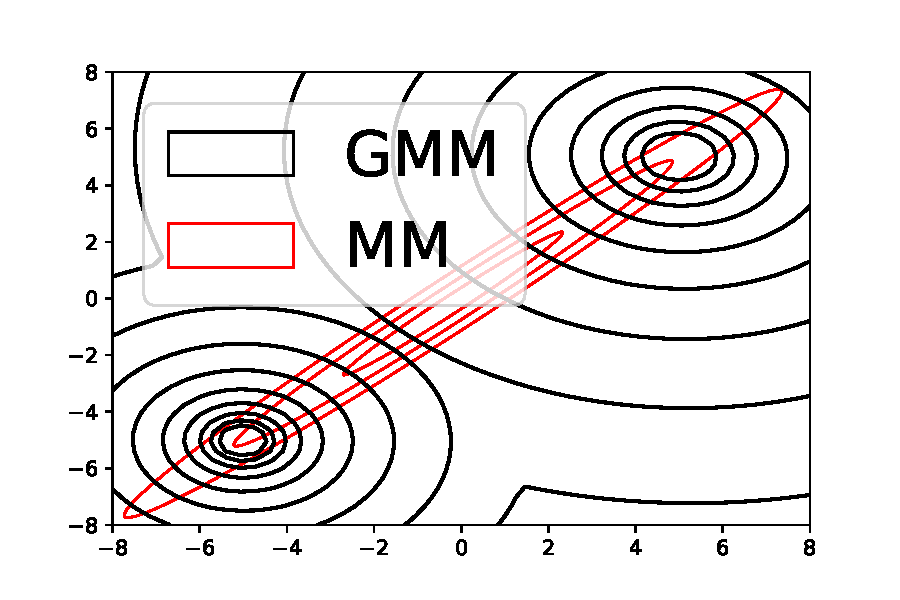
\includegraphics[width=.33\textwidth]{GMMContour.pdf}
%   }
%   \subfigure[Marginal pdf]{
%   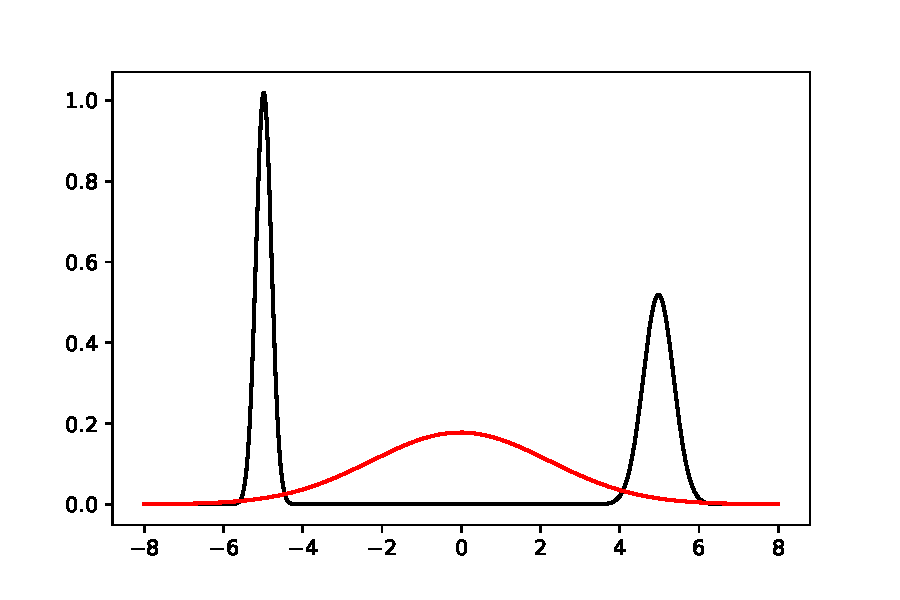
\includegraphics[width=.33\textwidth]{GMMpdf.pdf}
%   }
%   \subfigure[MI approximations]{
%   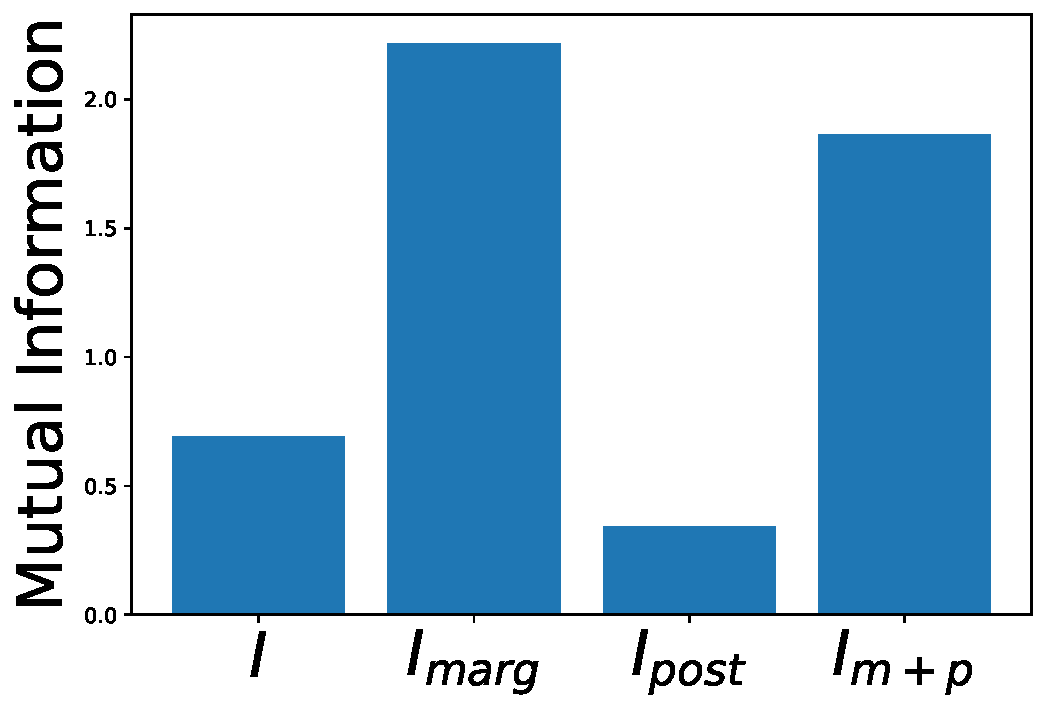
\includegraphics[width=.29\textwidth]{GMMbar.pdf}
%   }
%   \caption{\small\textbf{Moment Matched Gaussian Mixture Model} (a) A Gaussian Mixture 
%   Model with two means is plotted and its level curves. The moment matched 
%   Gaussian has its one standard deviation level curve plotted on top in red. (b)
%   The marginal pdf of the Latent Variable is plotted for the Gaussian Mixture 
%   Model and the moment matched Gaussian. The Gaussian is mean-seeking instead 
%   of mode seeking (c) The True $I(X,Y)$, $\Imarg(X,Y)$, $\Ipost(X,Y)$, and 
%   $\Iml(X,Y)$ are all plotted. Notice that $\Imarg(X,Y)\geq\Iml(X,Y)\geq\Ipost(X,Y)$ 
%   as expected.}
%   \label{fig:GMMex}
%   \end{figure*}

% \subsubsection{Equivalence of Methods}
% We first show that there exists a shared joint, $q(x,y)$, that generates 
% both $q_m$ and $q_p$. If this holds, then the stochastic gradient decent 
% approach can be reduced from minimzing two distribution to just one.\\

% \begin{lemma}{Uniqueness of Multivariate Gaussian}\\
%   For any linear conditional Gaussian variation distribution of the form 
%   $q(X|y)=N(Ay+b|\Sigma)$ where $\Sigma$ is independent of $y$, then there exists a 
%   unique joint Gaussian, $q(x,y)$, for any Gaussian marginal distribution $q(x)$.
%   \label{UniqueGaussian}
% \end{lemma}
% This tells us the assumption of $q_m$ and $q_p$ not sharing a joint Gaussian 
% is unnecessary as there exists a unique joint Gaussian that will produce any 
% separate $q_m$ and $q_p$. This reformulates equation ~\ref{eq:sgd_opt} To
% \begin{equation}
%   q^*(x,y) = \argmax_{q(x,y)}\left(\E_{p(x)}[\log(q(x))]+\E_{p(x,y)}(\log(q(x|y)))\right)
% \end{equation}

% \begin{theorem}{Equivalence of Moment Matching and Gradient Methods for Variational Gaussian}\\
%   Let $q_\eta(x,y)=N(\mu,\Sigma)$, $q_\eta(x)=\int q_\eta(x,y)dy$, 
%   and $q_\eta(x|y)=\dfrac{q_\eta(x,y)}{q_\eta(y)}$, where $\eta$ are the exponential 
%   family parameters of the joint Gaussian and $T(x,y)$ are the sufficient statistics. Then
% \[\E_{p(x,y)}[T(x,y)]=\E_{q(x,y)}[T(x,y)]\]
%   finds the same minimum as gradient ascent of
%   \[-\E_{p(x,y)}\left[log(q_\eta(x))+log(q_\eta(x|y))\right]\]
%   \label{EquivMethodsGauss}
% \end{theorem}

% The proof of Theorem \ref{EquivMethodsGauss} can be found in the appendix.\\ 
% Theorem~\ref{UniqueJoint} and Theorem~\ref{EquivMethodsGauss} together tell us 
% that if we are working with a Multivariate Gaussian variational distribution, 
% then Moment Matching is equivalent to Gradient Descent for minimizing the bound 
% in Theorem~\ref{thm:fosterbound}.\\

% \subsection{Properties of Variational Estimators}
% The $\Imarg$ and $\Ipost$ have nice properties that we can bound them relative 
% to the True MI. $\Iml$, on the other hand, is neither an upper bound or lower 
% bound due to bounding both entropy terms. However this approximation can be placed
% between the Variational Marginal and Variational Posterior bounds.\\
% \begin{lemma}
%   For any variational distributions $q_m(x)$ and $q_p(x|y)$, the following holds
%   \[\Ipost\leq\Iml\leq\Imarg\]
%   \label{lemma:MIOrder}
% \end{lemma}
% The proof of this lemma can be found in the appendix. However it is simple to see 
% that this must be true. The error of equation \ref{eq:mi_marg} is $KL(p(x)||q(x))$
% and the error of equation \ref{eq:mi_ml} is $KL(p(x)||q(x))-KL(p(x|y)||q(x|y))$ 
% which is error of the variational marginal minus a postive KL Divergence, 
% making it smaller than the upper bound. A similar argument holds to show that
% $\Iml$ is larger than the lower bound. \\
% Lemma ~\ref{lemma:MIOrder} always holds regardless of the model, however we can 
% ask when $\Iml$ is closer in absolute error to the true MI than either of the 
% bounds. Consider $\Ipost$, which has error $KL(p(x|y)||q(x|y))$
% \begin{equation}\label{eq:AbsPostError}
%   \left|KL(p(x|y)||q(x|y))\right|\geq \left|KL(p(x)|q(x))-KL(p(x|y)||q(x|y))\right| \Rightarrow 2KL(p(x|y)||q(x|y))\geq KL(p(x)||q(x))
% \end{equation}
% Equation ~\ref{eq:AbsPostError} shows us that $\Iml$ is closer in absolute error 
% to the true MI than $\Ipost$ if $2KL(p(x|y)||q(x|y))\geq KL(p(x)|| q(x))$. 
% Following a similar argument, $\Iml$ is close to the true MI than $\Imarg$ If
% $2KL(p(x)||q(x))\geq KL(p(x|y)||q(x|y))$. Neither of these conditions can be 
% checked in practice as True entropy terms need to be calculated to evalute these
% KL divergences, however this can be used to make Hueristic arguments for when $\Iml$ 
% is a good approximation. If $q(x)$ approximates $p(x)$ about as well as $q(x|y)$ 
% approximated $p(x|y)$, then $\Iml$ is better to use in all cases.\\
% \begin{figure*}[!htb]
%   \centering
%   \subfigure[Local minimum]{
%     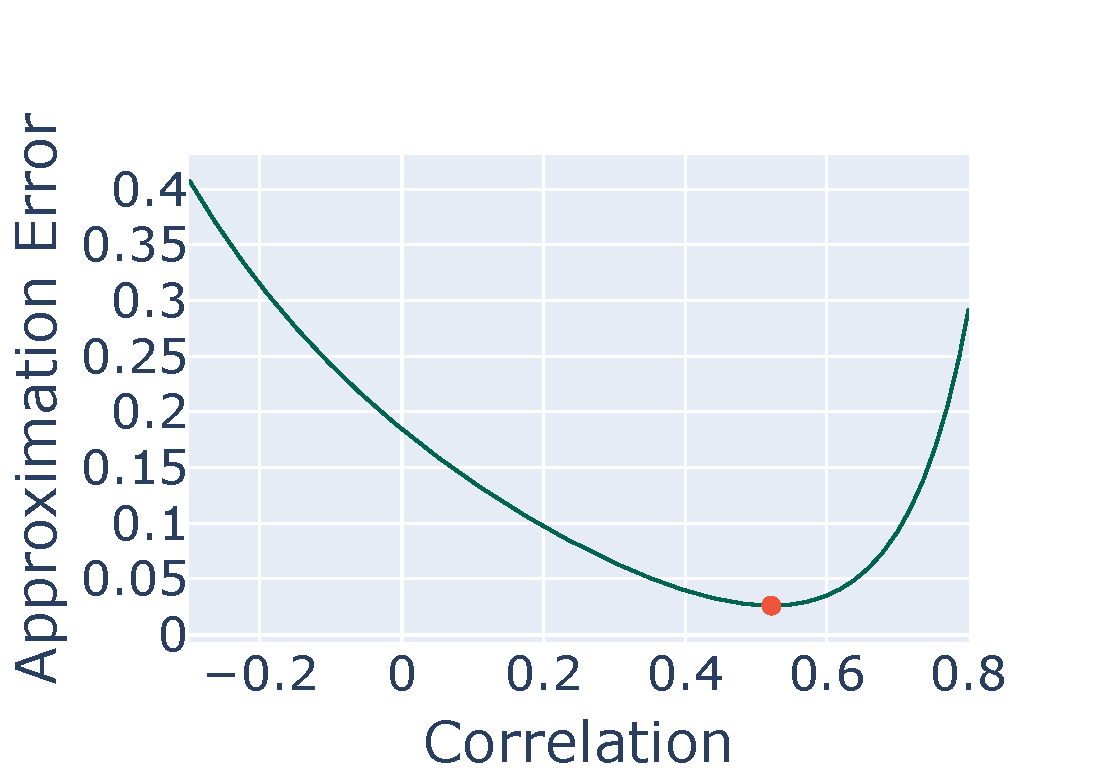
\includegraphics[width=.31\textwidth]{MMMinimum.pdf}
%     }
%   \subfigure[Local maximum]{
%   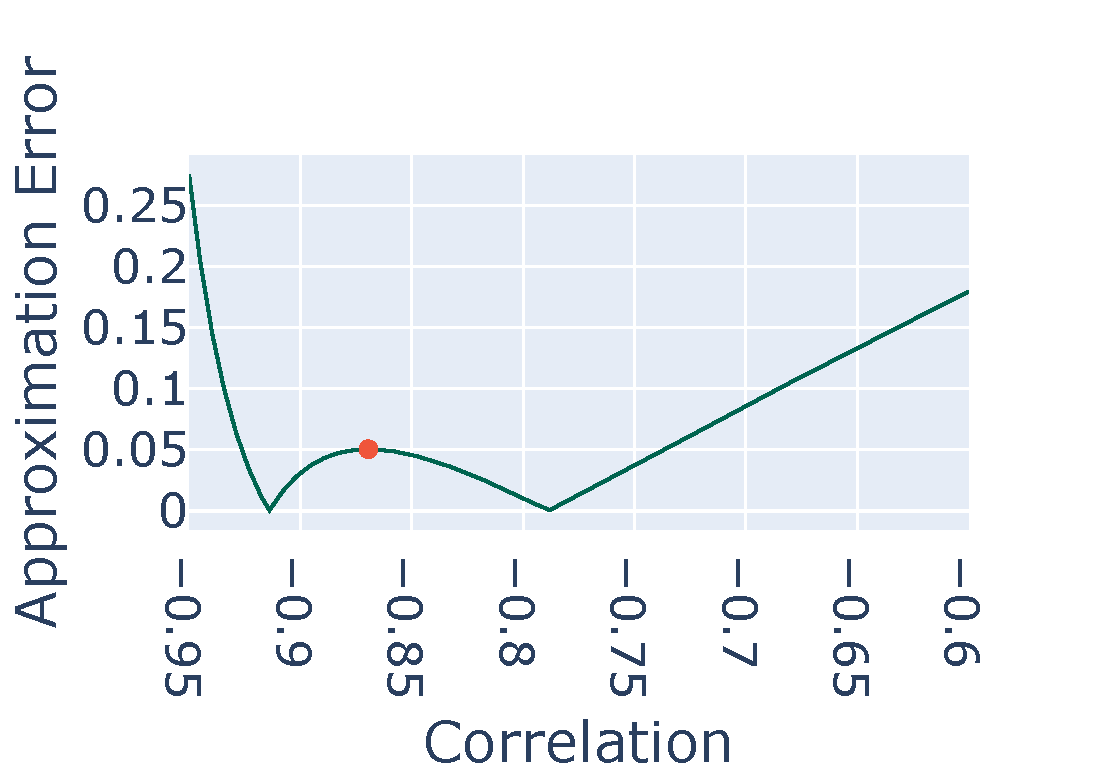
\includegraphics[width=.31\textwidth]{MMMaximum.pdf}
%   }
%   \caption{\small\textbf{Moment Matched Optimum} (a) In this case, a GMM is MM and then
%   the value of $\rho$ is varied. The Moment matching solution (red), is the local
%   minimum and no better values of $\rho$ exist. (b) Another GMM is MM, in this case
%   the moment matched solution finds a local maximum and there is a range of values
%   for $\rho$ that result in better approximation, and two that result in exact 
%   values of MI.}
%   \label{fig:MMoptimal}
%   \end{figure*}
% Another interesting property to note is that Moment Matching does not always find 
% a local minimum to the optimization of the variational distribution. Conisder 
% Figure ~\ref{fig:MMoptimal} where Gaussian Mixture Models are moment matched to a
% Gaussian. All of the paramters of the Moment Matched Gaussian is held constant but
% the correlation parameter, $\rho$, is plotted versus the absolute error to the True
% MI. In one case, the minimum is found and any changed value of $\rho$ results in a
% worse approximation of MI. However is the second case, a local maximum is found, 
% and we notice that there is a range of values for $\rho$ that result in not only
% better approximations of MI, but sometimes exact.\\

% \subsection{Optimizing $\Imarg$ and $\Ipost$}
% We now observe how to optimize Equation \ref{eq:mi_marg} and \ref{eq:mi_post}.
% Previously, the optimal distribution was found by minimizing the error $KL(p||q)$
% via a stochastic gradient methods, however, appealing to distributions in the 
% Exponential Family, this optimiziaiton can be simplified
% \begin{theorem}{Moment Matching Minimizes KL}
%   For any distribution, $p(x,y)$, and a Gaussian variational distribution, $q(x,y)$, 
%   the KL divergence, $KL(p(x)||q(x))$ and $KL(p(x|y)||q(x|y))$, are minimized 
%   by moment matching the joint.
%   \[E_p[T(x,y)]=E_q[T(x,y)]\]
%   \label{th:KLMin}
% \end{theorem}
% Because $\Imarg$ has an error of $KL(p(x)||q(x))$ and $\Ipost$ has an error 
% of $KL(p(x|y)||q(x|y))$, Moment Matching a Gaussian variational distribution 
% will minimze the $KL$ error of both methods and thus optimize the Variational 
% Marginal and Variational Posterior bounds. This means that when we moment match 
% a joint Gaussian, the resulting distribution will optimize $\Imarg$, $\Ipost$, 
% and $\Iml$ at the same time.

% \subsection{Generalize Proofs of Optimization}
% The results of Theorem \ref{UniqueGaussian} and Theorem \ref{EquivMethodsGauss}
% can be extended to include more general distributions as well. Theorem 
% \ref{UniqueGaussian} is extended in Seshadri and Patil \ref{SeshadriPatil}

% \begin{theorem}{Unique Joint Condition}\\
%   Given $f_x(x)$ and $f_{x|y}(x|y)$, a sufficient condition for
%   $f_y(y)$ (and hence for $f_{x,y}(x,y)$) to be unique is that the
%   conditional p.d.f. of $x$ given $y$ is of the exponential form
%   \[f_{x,y}(x|y)=exp\left[yA(x)+B(x)+C(y)\right]\]
%   where an interval is contained in the range of $A(x)$.
%   \label{UniqueJoint}
% \end{theorem}

% This generalizes the conditional distribution form being a linear Gaussian to 
% simply being in the exponential family and having a cross term tha tis linear 
% in $y$.\\
% Theorem \ref{EquivMethodsGauss} can be extend to further include other member of
% the exponential family.
% \begin{theorem}{Equivalence of Moment Matching and Stochastic Gradient Descent}
%   Let $q_m(x)$ and $q_p(x|y)$ share a common joint in the exponential family,

%   \[q_\eta(x,y)=h(x,y) \exp \left[\eta^TT(x,y)-A(\eta)\right]\]

%   Also assume linear conditional expectations of the sufficient statistics

%   \[\E_{q(x|y)}\left[T(x,y)\right]=\sum g_i(\eta)T_i(y)\hspace{2em} \E_{q(y|x)}\left[T(x,y)\right]=\sum h_i(\eta)T_i(x)\]

%   Then Moment Matching finds the same minimum as gradient ascent of Theorem \ref{thm:fosterbound}.
%   \label{EquivMethods}
% \end{theorem}


\section{Previous Work}\label{previousWork}
In this paper, we focused on the variational methods, $\Imarg$, $\Ipost$
~\cite{agakov2004algorithm}, and $\Iml$. The focus of each of these methods was 
computation speed ups for computing the optimal distribution. We also breifly 
discussed the Nested Monte Carlo estimator in \SEC\ref{background} and some of 
the challenges it faced. For each of these methods, Foster et al. 
~\cite{Foster2019} does a much more thorough analysis of convergence rate and 
run time. For an alternative implicit likelihood approximator, we also consider 
the likelihood-free inference by ratio (LFIRE) used by Kleinegesse and Gutmann 
~\cite{kleinegesse2021sequential} as a baseline for comparison purposes. For 
a general discussion of a variety of variational methods, a good resource is 
Poole et al ~\cite{poole2019variational} or Foster et al ~\cite{foster2020unified}.

%% In this section, methods to calculate mutual information and
%% variational methods will be discussed. There will be a overview of
%% each approach, however a deep analysis of each can be found in the
%% paper by Foster et al.~\cite{Foster2019}.

%% \subsection{Nested Monte Carlo}
%% The first approach is included from completeness but is a naive approach. 
%% Due to having neither $p(x|y)$ or $p(y)$ in closed form, sampling for Monte 
%% Carlo must be done twice in a nested manor.
%% \begin{equation}
%%   I(x,y)=\int\int p(x,y)\log \dfrac{p(y|x)}{p(y)}dxdy\approx\dfrac{1}{N}\sum_{n=1}^N \log\dfrac{p(y_n|x_{n,0})}{\dfrac{1}{M}\sum_{m=1}^Mp(y_n|x_{n,m})}
%% \end{equation}
%% where $x_{n,m}\sim p(x)$ and $y_n\approx p(y|x_{n,0})$. Here, $x$ is being 
%% marginalized out in the denominator to approximate $p(y)$.\\

%% \subsection{Variational Posterior}
%% The first variational method to discuss uses $q_p(x|y)$ to lower bound the 
%% posterior, $p(x|y)$. It was originally used by Barber and Agakov \cite{agakov2004algorithm} 
%% to bound mutual information for transmission on noisy channels.
%% \begin{definition}{Variational Posterior $I_{post}(x,y)$}\\
%%   \begin{equation}
%%     I_{post}(x,y)=\int\int p(x,y)\log\dfrac{q_p(x|y)}{p(x)}dxdy=H_p(p(x))-H_p(q(x|y))
%%   \end{equation}
%% \end{definition}

%% To compute this, a single MC estimator is needed

%% \begin{equation}
%%   I_{post}(x,y)=\int\int p(x,y)\log\dfrac{q_p(x|y)}{p(x)}dxdy \approx \dfrac{1}{N}\sum_{n=1}^N \log\dfrac{q_p(x_n|y_n)}{p(x_n)}
%% \end{equation}
%% where $x_n,y_n\sim p(x,y)$. To find the best variational distribution $q_p(x|y)$, 
%% one only needs to minimize the error given from Gibbs' Inequality

%% \[\min_{q_p}KL(p(x|y)||q_p(x|y))\]
%% Because KL is strictly non-negative, this error only occurs in one direction, 
%% giving us a bound. In the case of the Variational Posterior, this give a lower 
%% bound, so $I(X,Y)\geq I_{post}(x,y)$

%% \subsection{Variational Marginal}

%% The second variational method uses $q_m(y)$ to bound the predictive prior marginal. 

%% \begin{definition}{Variational Marginal $I_{marg}(x,y)$}\\
%%   \begin{equation}
%%     I_{marg}(x,y)=\int\int p(x,y)\log\dfrac{p(y|x)}{q_m(y)}dxdy =H_p(q_m(y))-H_p(p(y|x))
%%   \end{equation}
%% \end{definition}

%% Again, a single MC estimator is needed to compute this

%% \begin{equation}
%%   I_{marg}(x,y)=\int\int p(x,y)\log\dfrac{p(x|y)}{q_m(x)}dxdy \approx \dfrac{1}{N}\sum_{n=1}^N \log\dfrac{p(x_n|y_n)}{q_m(x_n)}
%% \end{equation}
%% where $x_n,y_n\sim p(x,y)$. To find the best variational distribution $q_m(x)$, 
%% one again only needs to minimize the error in Gibbs' Inequality 		
%% \[\min_{q_m}KL(p(x)||q_m(x))\]
%% This error give an upper bound on the true mutual information, 
%% so $I(X,Y)\leq I_{marg}(x,y)$

%% \subsection{Finding Optimal Varaitional Distributions}
%% In the case of both the Variational Posterior and Variational Marginal, 
%% we can directly approach minimizing the respective KL errors unlike the 
%% bounding need for the Impilcit Likelihood approximation. The standard 
%% approach to this is to use a gradient based optimizer to minimize both 
%% of these errors however, with slight modifications to Theorem~\ref{EquivMethods}, 
%% we can actually show that Moment Matching is again equivalent to minimizing 
%% the errorin the Gaussian case.
%% \begin{theorem}{Equivalence of Moment Matching and Gradient Methods}\\
%%   Let $q_\eta(x)=N(\mu,\Sigma)$ where $\eta$ are the exponential family parameters of the marginal Gaussian and $T(x)$ are the sufficient statistics. Then
%% \[\E_{p(x)}[T(x)]=\E_{q(x)}[T(x)]\]
%%   finds the same minimum as gradient ascent of
%%   \[\min_{q_m}KL(p(x)||q_m(x))\]
%%   Likewise, let $q_\eta(x|y)=N(Ay+b,\Sigma)$ where $\eta$ are the exponential family parameters of the joint Gaussian and $T(x,y)$ are the sufficient statistics. Then
%% \[\E_{p(x,y)}[T(x,y)]=\E_{q(x,y)}[T(x,y)]\]
%%   finds the same minimum as gradient ascent of
%%   \[\min_{q_p}KL(p(x|y)||q_p(x|y))\]
%%   \label{EquivMethodMargPost}
%% \end{theorem}\
%% The proof of Theorem~\ref{EquivMethodMargPost} is near identical to that 
%% of Theorem~\ref{EquivMethods} just with the argument broken up. This will 
%% be included in the appendix for completeness.



\section{Experiments}\label{experiments}
We demonstrate efficacy and efficiency of our moment matching
variational MI estimators in a range of experiments beginning with a
Gaussian mixture model (\SEC\ref{sec:gmm}).  We then evaluate two
implicit likelihood models: one arising from the non-closed-form
marginalization of nuisance variables in a GLM
(\SEC\ref{sec:extrapolation}), and the other is a simulation-based SIR
epidemiology model (\SEC\ref{sec:sir}).  In all cases we find that the
proposed moment matching estimators offer substantial computational
speedups while achieving identical MI bounds and approximations to
existing methods.

%% A variety of experiments are used to demonstrate the efficiency of the 
%% Moment Matching of the Implicit Likelihood approximation compared to a 
%% variety of other approaches. The experiments chosen are joint 
%% multivariate Gaussian Mixture Model, and implicit extrapolation setting,
%% and SIR parameter estimation. We demonstrate two major takeaways. First, 
%% Moment Matching is substantially faster than Gradient based approaches 
%% for finding optimal variational distributions and second, we show that 
%% the Implicit Likelihood approximation does not sacrifice accuracy of 
%% approximation compared to Variational Posterior or Variational Marginal, 
%% which assumes exact marginal entropy or exact posterior calculation, 
%% respectively.

% \subsection{A/B Test}
% \begin{figure*}[!htb]
    \centering
    \subfigure[MI by Decision]{
    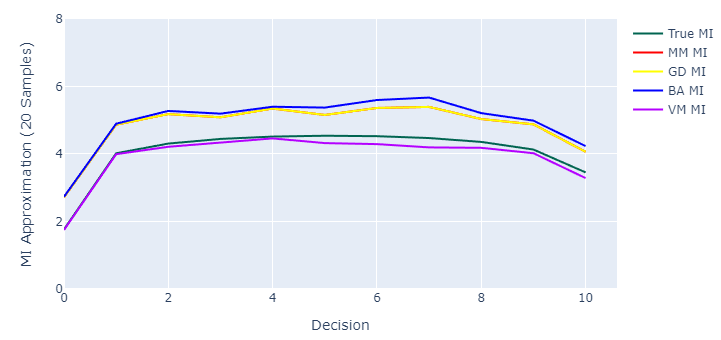
\includegraphics[width=.48\textwidth]{ABMI20.png}
    }
    \subfigure[Gradient Step Convergence]{
    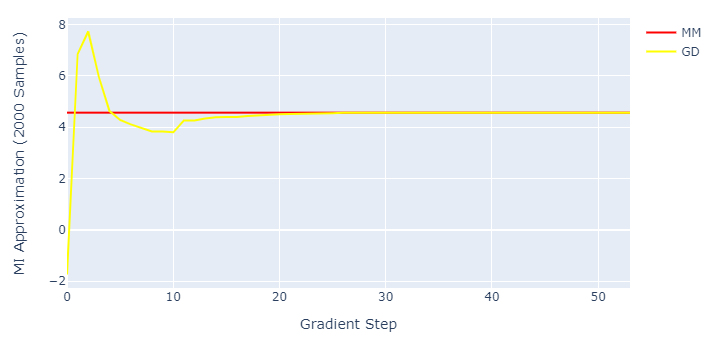
\includegraphics[width=.47\textwidth]{ABGDStep.png}
    }
    \caption{\textbf{A/B Test} for $11$ decisions of assigning $10$ participants to $2$ groups. Because the method is Gaussian linear, each model converges to the true Mutual Information. (a) $20$ samples were used to compute the mutual Information for each decision (b) This plot shows the convergence of the Gradient Descent approach approximation with respect to the number of Gradient Steps. Notice that the Gradient step converges to the Moment Matching Solution but takes $~50$ steps. The Moment Matching reaches this end convergence immediately without needing to do multiple evaluations.}
    \label{fig:ABDGStep}
    \end{figure*}
    
    We consider the classical A/B test with a Gaussian linear model. The experiment 
    in this case is where $D$ participants are chosen to be split into two 
    groups, $A$ and $B$. The design is the choice of the group size, $d_A$ for 
    group $A$ and $d_B=N-d_A$ for group $B$. Each participant then has a measured 
    continuous response $y$. The Bayesian model is a Gaussian linear as follows.
    \begin{equation}
    x\sim N(0,\Sigma_x)\hspace{2em} y|x,d \sim N(D_dx,I)\hspace{2em}\Sigma_x = \begin{bmatrix}
    10^2 & 0 \\
    0 & 1.82^2
    \end{bmatrix}
    \end{equation}
    where $D_d$ is the design matrix of size $D\times 2$ with the first $d_A$ rows 
    as $(1,0)$ and the remaining as $(0,1)$ to signify group assignments. For this 
    experiment, we will us $D=10$ participants.\\
    For variational distribution, we assumed linear multivariate gaussians from 
    the Exponential Family for both the marginal and likelihood. To evaluate each 
    approximation, $N$ samples are drawn from the prior and then the posterior 
    as $x_n\sim p(x)$ and $y_n\sim p(y|x=x_n)$.\\
    
    Figure \ref{fig:ABDGStep} shows the evaluations of Moment Matching, Gradient 
    Descent, Variational Posterior, and Variational Marginal to the true Mutual 
    Information $N=20$ Sample Points. Notice, the Moment Matching and Gradient 
    Descent Approach both match for each decision evaluation as expeceted. In 
    Figure  \ref{fig:ABDGStep}, we compare the Mutual Information evaluation of 
    Moment Matching to that of Gradient Descent with respect to gradient steps. 
    Notice that Gradient Descent approaches the Moment match solution but take 
    approximately K step before it has leveled out.\\
    
    Another important property to observe from the Figure \ref{fig:ABDGStep} is 
    that the theoretical bound have been swapped for Varaitional Posterior and 
    Variational Marginal distributions, that is Variational Marginal should be 
    an upper bound but is a lower bound and vice-versa. This is due to a bias 
    introduced from finite sample plug in estimators. It is easily shown 
    that $\E[\hat{\Sigma}]=\frac{n+1}{n-1}\Sigma$. So in this case where our 
    variational distributions are the same family as the target distributions 
    (Gaussian), the error bound from Gibbs' inequality is less than that of the 
    introduced bias and the bound swaps. For examples where the target distribution 
    is not a Gaussian, the bias tends to be negligible compared to the approximation 
    bound.\\
    
    For further analysis, Figure \ref{fig:ABConvergence}, the convergence rate and 
    time of each method is shown for the decision with the maximum Mutual 
    Information ($d=5$) with respect to the number of samples taken. We notice after 
    a few hundred samples, all of the methods have converged to the true Mutual 
    Information. We also see that for computation time, every method is orders of 
    magnitude faster than that of the Gradient Descent. We will see that as the 
    dimensionality of the problem increases, the speed of Moment Matching will be 
    highlighted in comparison to Variational Marginal and Variational Posterior.
    
    \begin{figure*}[!htb]
    \centering
    \subfigure[MI Convergence]{
    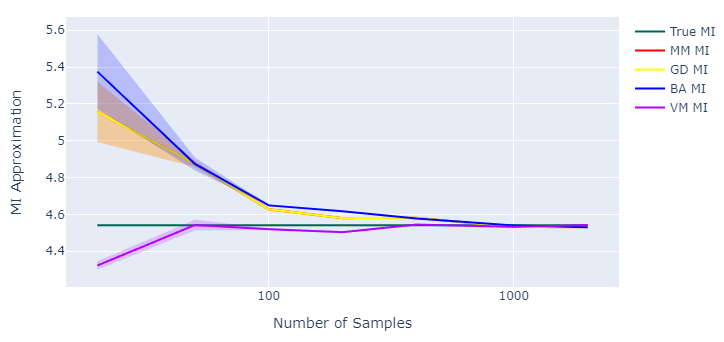
\includegraphics[width=.48\textwidth]{ABConverge.png}
    }
    \subfigure[Computation Time]{
    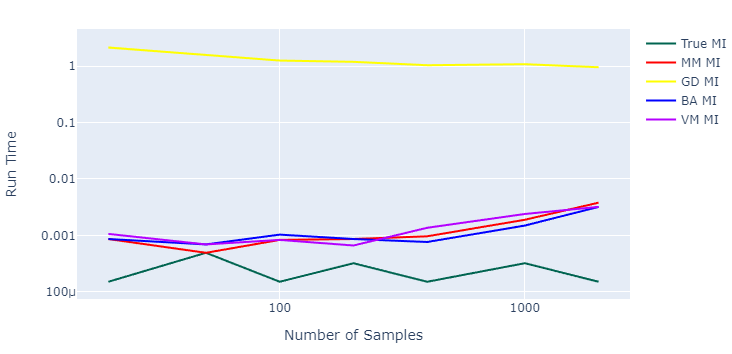
\includegraphics[width=.47\textwidth]{ABTime.png}
    }
    \caption{\textbf{A/B Test Mutual Information Estimation} for $11$ decisions of assigning $10$ participants to $2$ groups. Because the method is Gaussian linear, each model converges to the true Mutual Information. (a) The convergence of MI with respect to the number of samples drawn is plotted for the maximum MI decision ($d=5$) (b) The run time of each method is plotted for the number of samples for the maximum MI decision ($d=5$). Note that Moment Matching and Gradient Descent Match in approximation Value however Moment matching save orders of magnitude in computation time. }
    \label{fig:ABConvergence}
    \end{figure*}

\subsection{Multivariate Gaussian Mixture Model}\label{sec:gmm}
GMMs are pervasive in statistics due to their universal approximation
properties, yet calculating MI for a GMM is notoriously
challenging~\cite{huber2008entropy}.  In this section we extend the
two-dimensional example (\FIG\ref{fig:GMMex}) to high-dimensional
GMMs.  We simulate a bivariate GMM,
\begin{equation}
  p(x,y) = \omega \Ncal(m_0, \Sigma_0) + (1-\omega) \Ncal(m_1, \Sigma_1)
\end{equation}
with $\omega \in [0, 1]$ and dimensions $X \in \mathbb{R}^{100}$ and
$Y \in \mathbb{R}^{200}$.  We use this setting to demonstrate
efficient MI estimation even in very high-dimensional distributions.

\FIG\ref{fig:LargeGMMConvergence} shows substantial speedups in
runtime (left) for all methods as compared to gradient optimizatoin
(center).  Notice that GD takes approximately 2000 gradient steps to
converge for $5,000$ samples whereas moment matching found this
solution immediately, independ of any gradient steps.  As per our
theoretical results we find that $\Iml$ always lies between the MI
upper bound $\Imarg$ and lower bound $\Ipost$ with $\Imarg$ being most
accurate estimator in this model (right).
\begin{figure*}[t]
  \centering
  \begin{tabular}{ccc}
    \hspace*{-4mm}\subfigure[Computation Time]{
    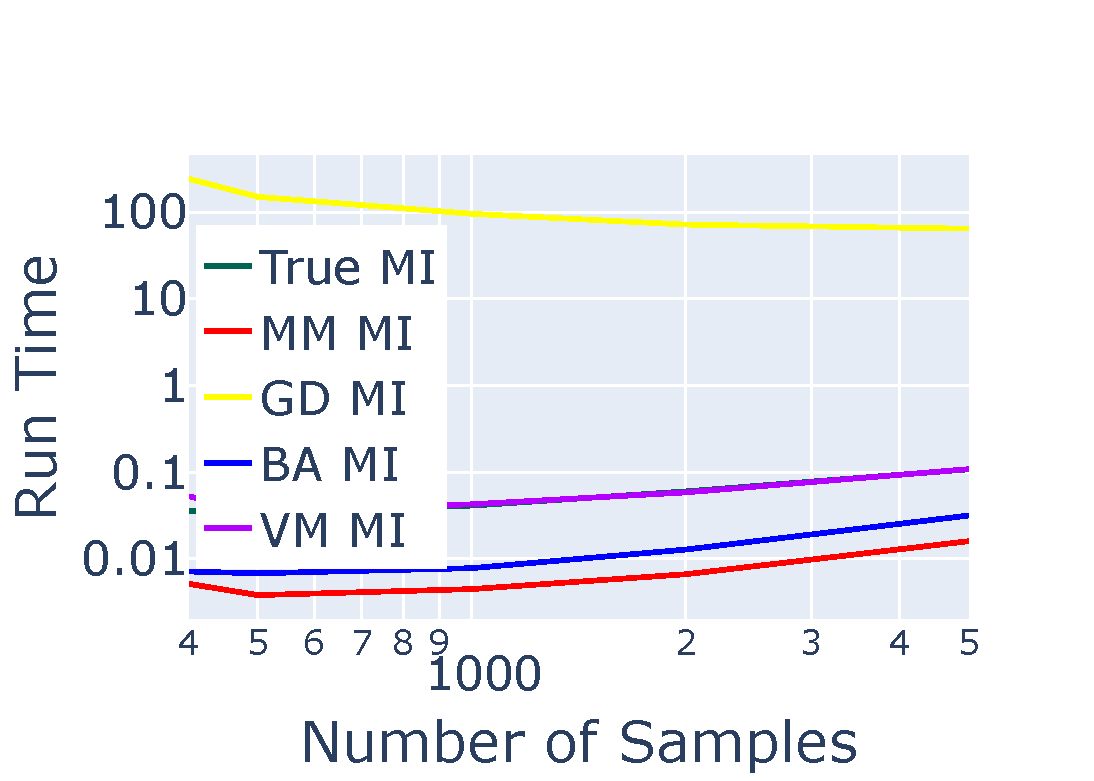
\includegraphics[width=.36\textwidth]{LargeGMMTime.pdf}
    }
    \hspace*{-6mm}\subfigure[GD Convergence]{
        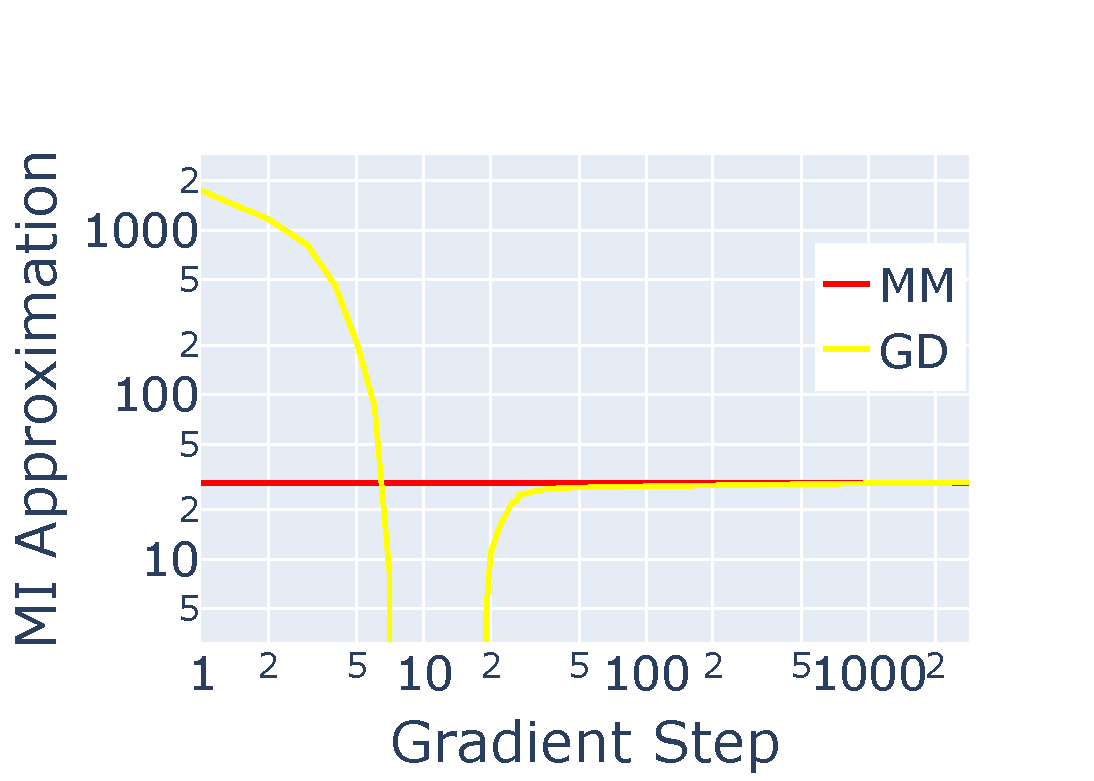
\includegraphics[width=.36\textwidth]{GMMGDStep.pdf}
    }    
    \hspace*{-6mm}\subfigure[MI Convergence]{
    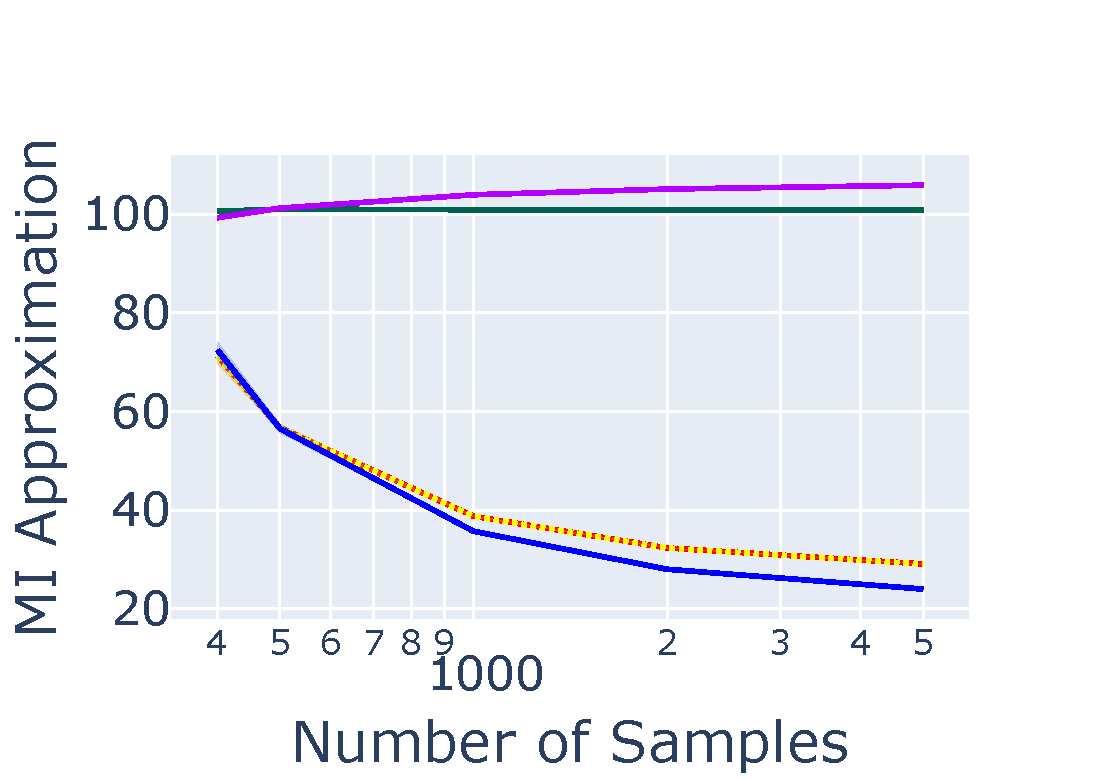
\includegraphics[width=.36\textwidth]{LargeGMMConverge.pdf}
    }
  \end{tabular}
    \caption{\small\textbf{High-dimensional Bimodal GMM.} Moment
      matching estimates have orders of magnitude lower computation as
      a function of sample size (a).  As per our theoretical analysis,
      our moment-matching solution to $\Iml$ achieves the same
      estimate while avoiding gradient iterations (b).  In this model
      we see that $\Imarg$ yields the most accurate estimates.  ``True
      MI'' is calculated via Monte Carlo estimation with exact
      evaluation of the model probabilities.}
    \label{fig:LargeGMMConvergence}
    \end{figure*}

%% sample convergence (right) for each method. We see that each
%% approximation satisfies the theoretical bounds discussed, with
%% $\Ipost$ as a lower bound, $\Imarg$ as an upper bound, and $\Iml$
%% lying inbetween. We can observe the computation times in this high
%% dimensional case. The true MI is more computationally intensive in
%% this scenario so we see that Moment Matching is slighly faster than
%% computing $\Imarg$ and $\Ipost$.

%% A synthetic model is constructed for explicit comparing of methods. In these 
%% experiments, a multivariate Gaussian Mixture Model with $K$ modes, latent 
%% variable dimension $D_x$, and observation variable dimension $D_y$ , is generated 
%% as the joint distribution. Samples can be directly drawn from the prior and 
%% then the posterior as $x_n\sim p(x)$ and $y_n\sim p(y|x=x_n)$. Since the true 
%% distributions are known, the true entropy can be numerically calculated using 
%% these samples. We will compare each of the methods to this numerical calculation.\\

%% The GMM we will consider will have high dimensions, with $K=2$, $D_x=100$ 
%% and $D_y = 200$. The purpose of this will be to emphasis the efficiency of 
%% calculating MM approximation over the Varaitional Marginal, Variational Posterior,
%% and especially over Gradient Descent. \\

%% Most importantly, moment matching is orders of magnitude faster than
%% computing the Gradient Descent approach for the exact same
%% approximation. To emphasis this result, consider the convergence of
%% gradient descent in Figure \ref{fig:LargeGMMConvergence}
%% (right). 

%% Using Moment Mathcing for $\Iml$, notice that we get similar quality approximations
%% to MI while saving drastic compution time. In a scenario with even higher 
%% dimensionality or a large domain of decisions, the computational speed up of Moment
%% Matching is drastic compared to $\Imarg$, $\Ipost$, and especially $\hat{I}_{NMC}$.


% \begin{figure*}[!htb]
%     \centering
%     \subfigure[MI Convergence]{
%     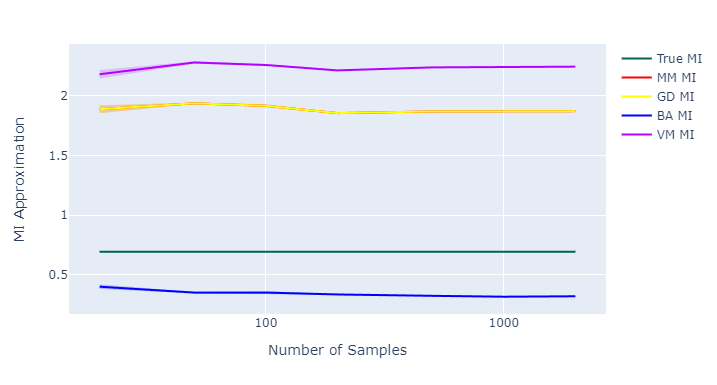
\includegraphics[width=.34\textwidth]{GMMMI.png}
%     }
%     \subfigure[Computation Time]{
%     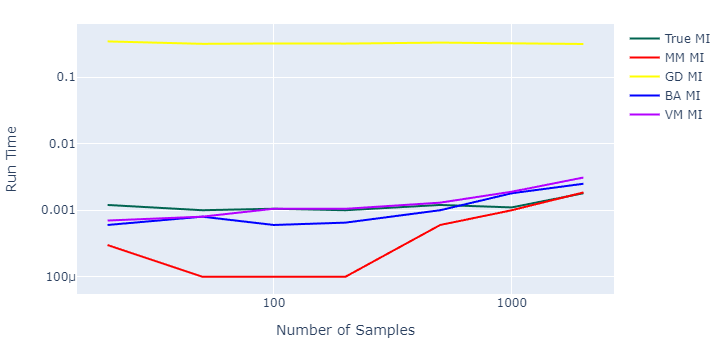
\includegraphics[width=.34\textwidth]{GMMTime.png}
%     }
%     \subfigure[Samples]{
%     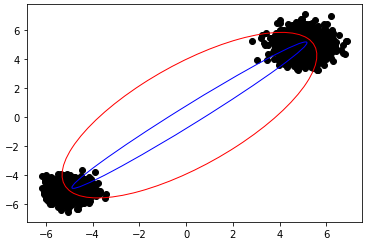
\includegraphics[width=.26\textwidth]{GMMSample.png}
%     }
%     \caption{\textbf{Gaussian Mixture Model Mutual Information Estimation} A Guassian Mixture model with 2 modes and Dimensions of Latent Variable, $X$, and Observation Variable $Y$, both being $1$. (a) The convergence of MI with respect to the number of samples drawn is plotted (b) The run time of each method is plotted for the number of samples. (c) The plotted samples drawn with an overlayed Moment Matched Gaussian Variational Approximation and an "Oracle" Gaussian approximation that matches the true Mutual Information. Variational Marginal is and upper bound, Variational Posterior is a lwoer bound, and MM/GD is a closer upper bound.}
%     \label{fig:GMMConvergence}
%     \end{figure*}
% Likewise, we can compute and "oracle" variational distribution which learns 
% it parameters by minimizing the absolute difference in the numerical Mutual 
% Information to the Implicit Likelihood approximation. This will be used to 
% qualitatively compare against the learned moment matching distribution.
% The first GMM we will consider will have $K=2$, $D_x=1$, and $D_y=1$. 
% Figure \ref{fig:GMMConvergence} show the convergence rate and time of each 
% methods. Now that our model is no longer linear gaussian, we see that the bound 
% of each methods holds as the bias introduced due to the plug in estimator is 
% negligible with respect to the varitional bounds. We again notice that each 
% method is significantly faster than that of the Gradient Descent.\\

% Figure \ref{fig:GMMConvergence} shows the sampled points along with the 
% Moment Match distribution and the Oracle distribution. We notice that both 
% share many similar quantities however the Oracle is a has larger variance 
% in on direction. This is responsible for lowering the Mutual Information to 
% match the True Mutual information by creating more uncertainty in the added 
% variance. This shows where the information is lost in Moment Matching for this 
% example.\\


\subsection{Extrapolation}\label{sec:extrapolation}
\begin{figure*}[!t]
    \centering
    \hspace*{-5mm}\subfigure[MI Convergence]{
      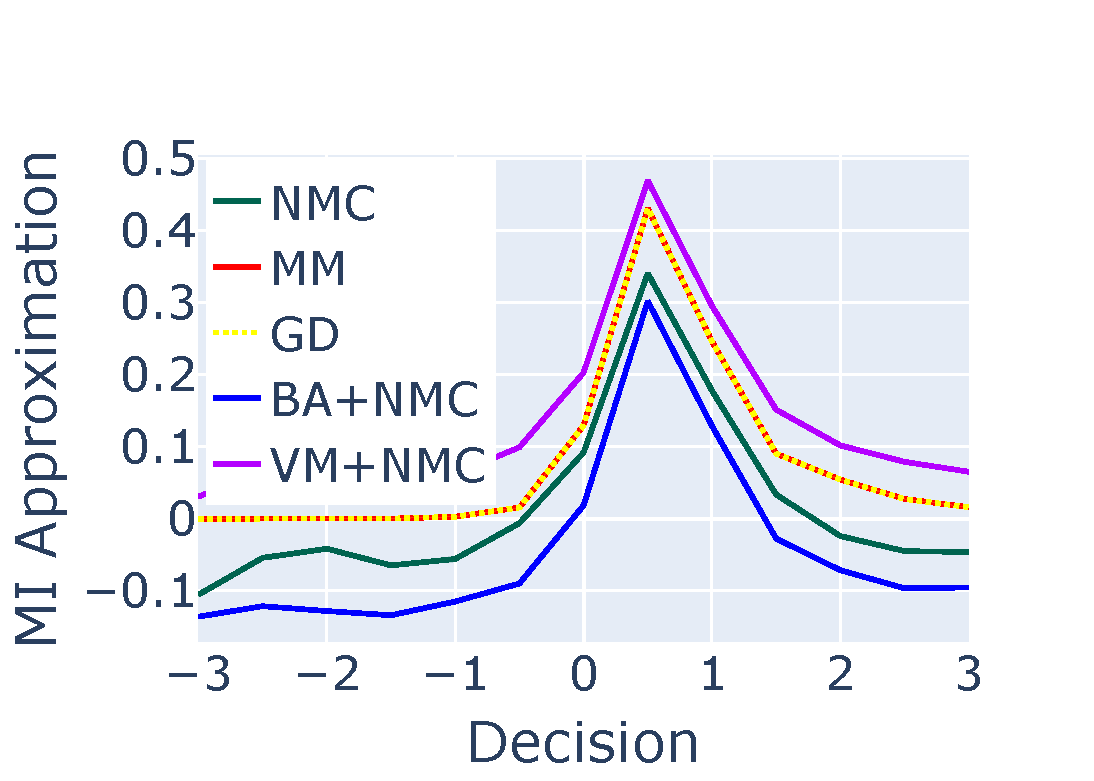
\includegraphics[width=.36\textwidth]{ExtrapolationMI.pdf}
    }
    \hspace*{-7mm}\subfigure[Computation Time]{
      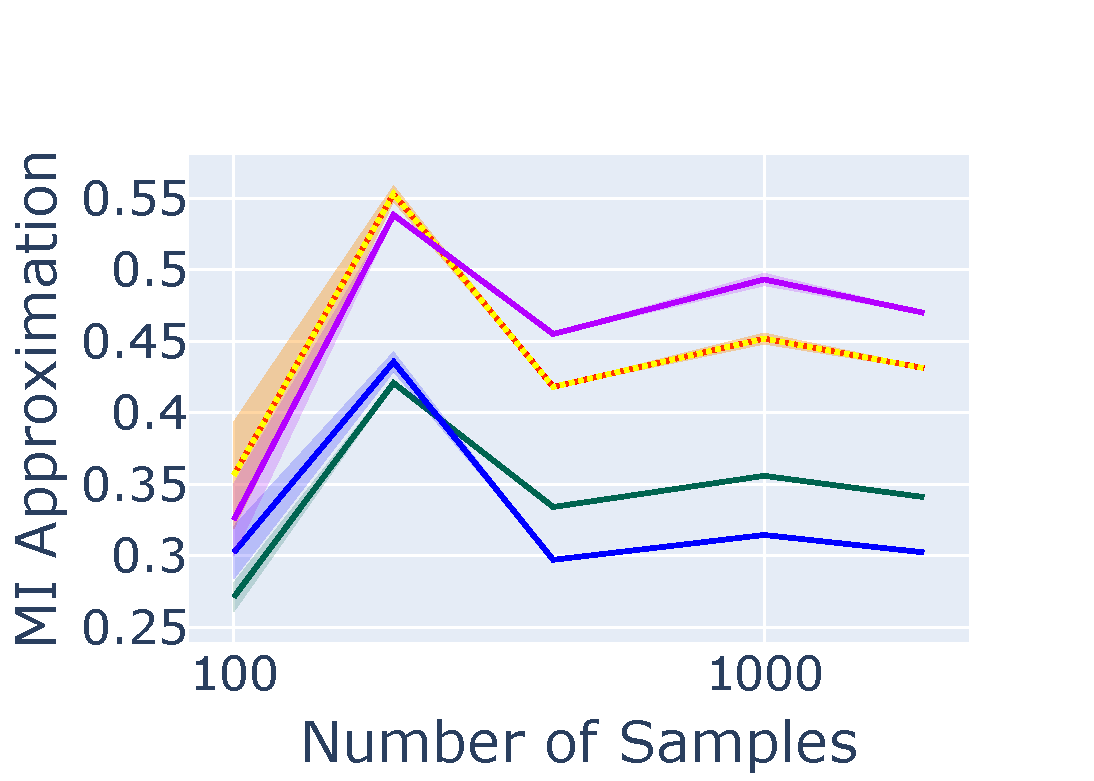
\includegraphics[width=.36\textwidth]{ExtrapolationConverge.pdf}
    }
    \hspace*{-7mm}\subfigure[Samples]{
      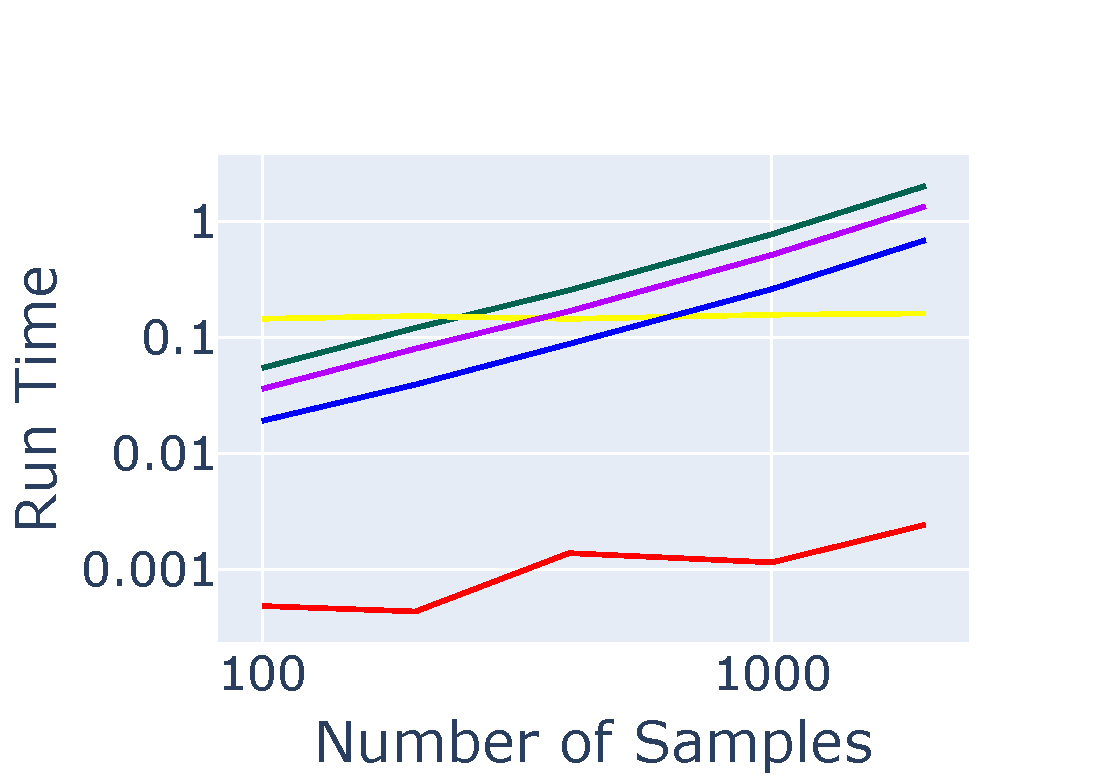
\includegraphics[width=.36\textwidth]{ExtrapolationTime.pdf}
    }
    \caption{\small \textbf{Extrapolation} (a) The MI for decisions $d
      \in [-3,3]$ with variances $\sigma_x^2 = 3$, and $\sigma_y^2=1$
      for each approximation with 4000 samples is plotted with $d=.5$
      being the maximum. Note the negative bias resulting from
      NMC. (b) The convergence rate versus samples is plotted at
      maximum decision ($d=.5$) (c) The run time for each method is
      plotted with moment matching being orders of magnitude faster than
      any other method.}
    \label{fig:Extrapolation}
\end{figure*}

We adapt the following experiment from Foster et
al.~(\citeyear{Foster2019}) intended to evaluate the implicit
likelihood MI estimator $\Iml$ (or $\hat{I}_{m+\ell}$).  Labeled
information, $y$, from a subset of the design space is be used to
predict labels at a location $x$ that can't be directly observed. The
model is as follows,
\[
 \psi\sim \Ncal(\mu_\psi, \Sigma_\psi), \quad  \theta \mid \psi \sim \Ncal\left( (X_\theta^T \psi)^2, \sigma_x^2 \right) \quad y\mid\psi,d \sim \Ncal\left( (X_d^T \psi)^2, \sigma_y^2 \right)
\]
where $X_x = (1,-\frac{1}{2})$ and $X_d = (-1,d)$.  The aim is to
choose a design $d \in \mathbb{R}$ that maximizes $I(\theta ; Y \mid
d)$.  Thus, $\psi$ is a nuisance variable that must be marginalized.
This marginalization lacks a closed-form and so the likelihood $p(y
\mid \theta)$ is implicit--it cannot be evaluated nor efficiently
sampled.  As a baseline we draw $N$ samples from the joint and use the
NMC estimator to compute entropies as:
\begin{equation}
    H(\theta)= -\int p(\theta)\log(p(\theta))dx \approx -\dfrac{1}{N}\sum_i \log\left(\dfrac{1}{N-1}\sum_{j\neq i}p(\theta_i|\psi_j)\right)
    \label{eq:NMCentropy}
\end{equation}
%% To compute each of these methods, we will sample from $x_i,y_i,\psi_i
%% \sim p(\psi)p(x|\psi)p(y|\psi,y)$ and we will need to compute a NMC
%% estimator for the $H_p(p)$ terms in $\Imarg$ and $\Ipost$ as well as
%% for a total approximation of $I(X,Y)\approx I_{NMC}(X,Y)$. To compute
%% each entropy term from samples, we use

\FIG\ref{fig:Extrapolation} summarizes the proposed estimators and
runtime.  As the theory suggests our moment matching estimators
provide substantial speedup, and we observe accurate estimates with
$\Iml$ in this model.  We emphasize that $\Imarg$ and $\Ipost$ are
infeasible due to the need to estimate model entropies in this
implicit likelihood model.  We instead augment these methods with the
NMC estimator (e.g. \EQN\eqref{eq:NMCentropy}), which is referred to
as \emph{variational NMC} in the literature~\cite{Foster2019}.
However, the finite sample bias of NMC violates expected bound
properties for few samples--see \FIG\ref{fig:Extrapolation} (center).
We include these estimators to highlight the difficulty of estimating
MI in implicit likelihood models and to emphasize their practical
limitations.

%% An issue with this approximation is that despite it being consisent, it is biased
%% and the bias decays slowly (Zheng, 2018). When we observe Figure
%% ~\ref{fig:Extrapolation}(a)(b), we notice that the NMC is negative for some 
%% values of $d$. $I(X,Y)\geq0$ so this is the effect of the bias. Likewise, since 
%% the Variational Posterior and Variatoinal Marginal use entropy terms computed
%% using the NMC, they too are biased. However, we do notice that we maintain the 
%% ordering of the approximators from Lemma~\ref{lemma:MIOrder}.\\
%% From the experiment, we see that the optimal decision is when $d=.5$. This makes
%% intuitive sense for our problem as $X_x=(1,-\frac{1}{2})$ and 
%% $X_d = (-1,\frac{1}{2})$ which implies that they are highley negatively 
%% correlated, giving infromation about one another. As for the run time in (c), we
%% notice that Moment Matching is uniformaly faster than any other method by a few
%% orders of magnitude. Also, after approximatley 500 samples, the gradient decsent
%% based method becomes computationally cheaper than the NMC methods.\\
%% From this experiment, we see that moment matching provides a qualitatively good 
%% estimation as any other method while simulateously saving orders of magnitude in
%% computation time.\\


\subsection{SIR Epidemic Model}\label{sec:sir}
\begin{figure*}[t!]
  \centering
  \hspace{-8mm}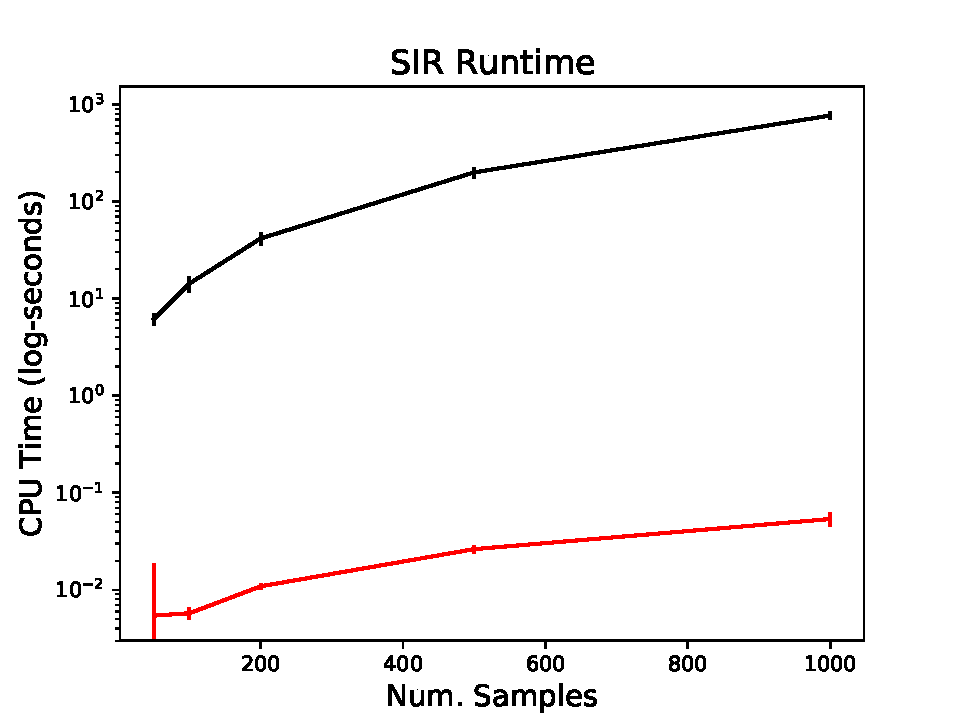
\includegraphics[width=0.28\textwidth]{sir_runtime_benchmark}
  \hspace{-4mm}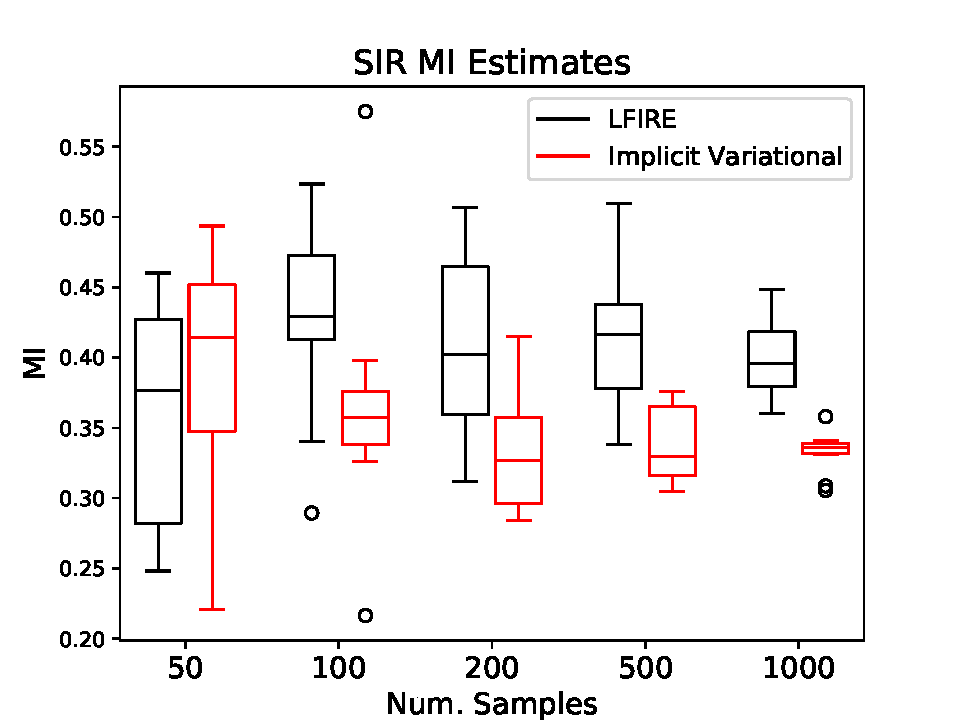
\includegraphics[width=0.28\textwidth]{sir_utility_benchmark}
  \hspace{-4mm}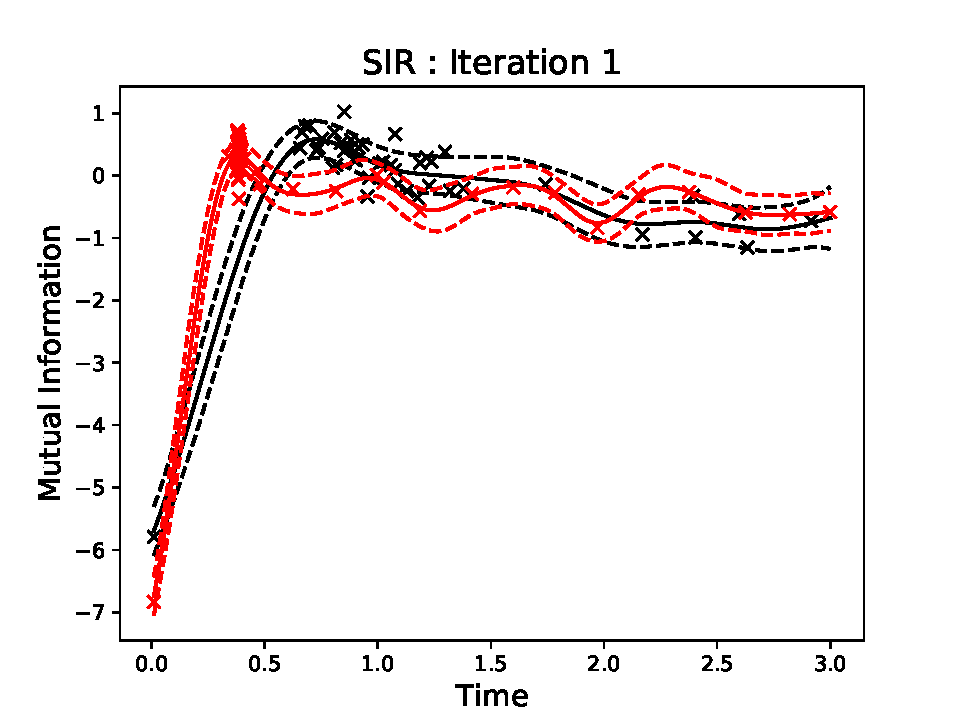
\includegraphics[width=0.28\textwidth]{sir_500p_K3_iter1}
  \hspace{-4mm}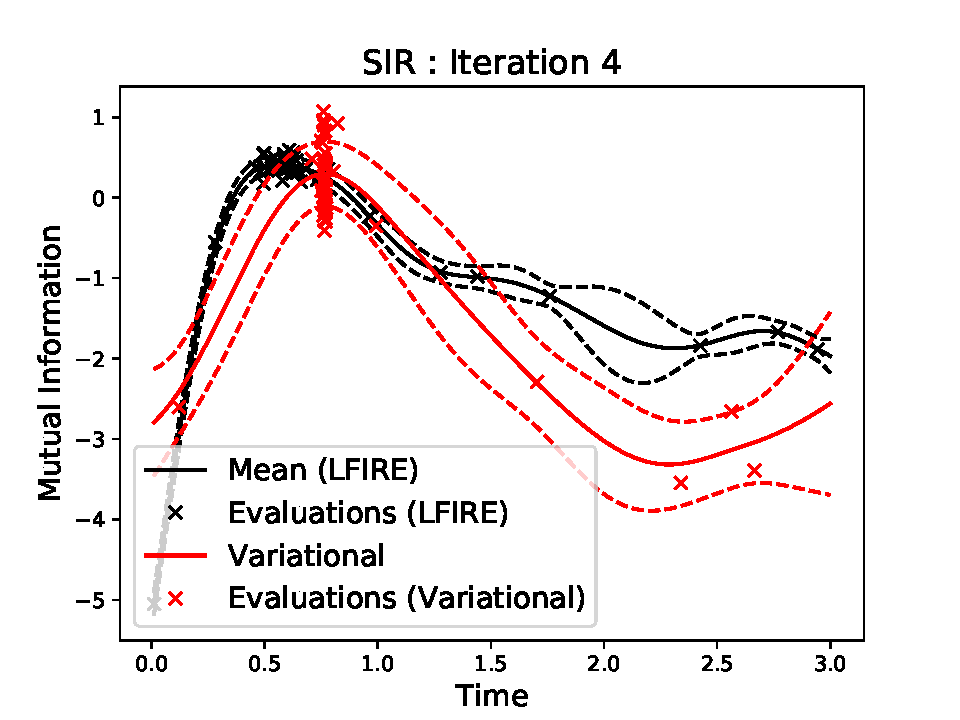
\includegraphics[width=0.28\textwidth]{sir_500p_K3_iter4}
  \caption{\small \textbf{SIR Sequetial Design.} Left plots show benchmark
    time and utility evaluation between LFIRE and the Variational
    estimator for a fixed design ($d=1.0s$) over 10 runs each at a
    range of sample sizes.  The variational estimator is orders of
    magnitude more efficient (\emph{left}) and shows lower variance at
    each sample (\emph{center-left}).  The first (\emph{center-right})
    and fourth (\emph{right}) sequential BED iterations yield
    comparable designs between both methods (GP posterior MI shown).}
  \label{fig:sir_results}
\end{figure*}

\paragraph{The SIR model} 
describes the time-evolution of infection in a fixed
population~\cite{kermack1927contribution, allen2008introduction}.  At
each time $t$ the population is divided into three components:
\emph{susceptible} $S(t)$, \emph{infected} $I(t)$, and
\emph{recovered} $R(t)$ according to the time-series,
\begin{align}
  S(t + \Delta_t) &= S(t) - \Delta I(t) \label{eq:s} \\
  I(t + \Delta_t) &= I(t) + \Delta I(t) - \Delta R(t) \\
  R(t + \Delta_t) &= R(t) + \Delta R(t) \label{eq:r}
\end{align}
\begin{wrapfigure}{r}{0.3\textwidth}
  \vspace*{-5mm}
  \centering
  \hspace*{-5mm}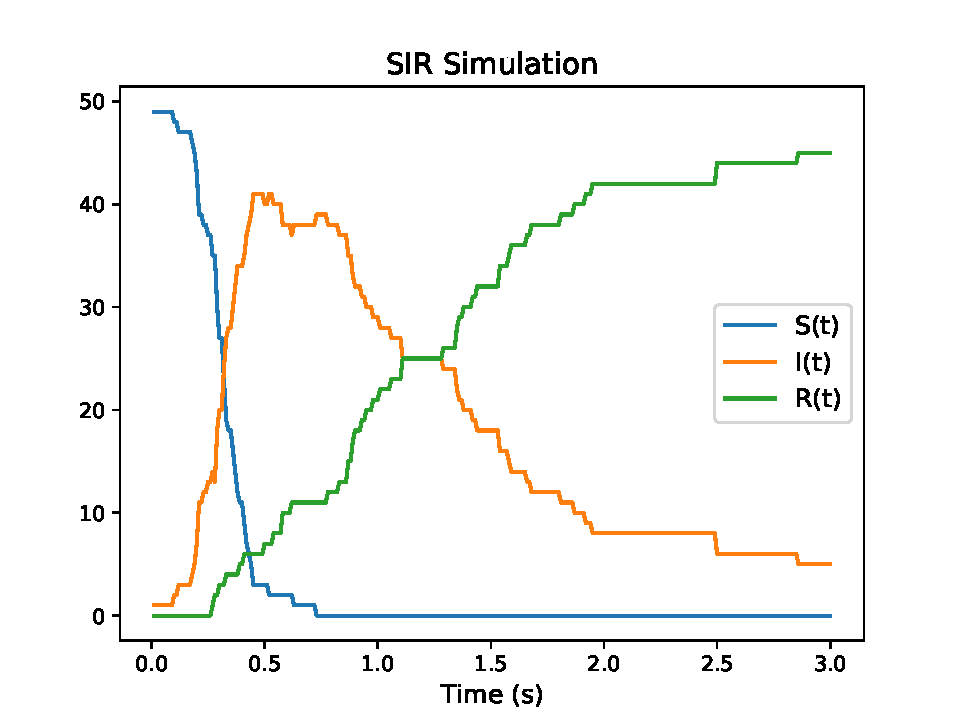
\includegraphics[width=0.35\textwidth]{sir_sim_beta_0p14_gamma_0p01}  
  \caption{\small SIR model simulation for $\beta = 0.14,
    \gamma=0.01$.}
  \vspace*{-5mm}
  \label{fig:sir_sim}
\end{wrapfigure}
At each time the change in infected $\Delta I(t)$ and recovered
$\Delta R(t)$ are Binomially distributed,
\[
  \Delta I(t) \sim \text{Binomial}\left(S(t), \frac{\beta
    I(t)}{N}\right), \quad
  \Delta R(t) \sim \text{Binomial}(I(t), \gamma)
\]
with unknown random parameters $\beta, \gamma \sim
\text{Uniform}(0,0.5)$.  Our simulations use a fixed discrete time
interval $\Delta_t = 0.01$ with a population $N=50$ and boundary
conditions $S(t=0) = N-1$, $I(t=0)=1$, and $R(t=0) =
0$. See \FIG\ref{fig:sir_sim} for an example of the SIR simulation.


\paragraph{Sequential Design} We select a time $t > 0$ with maximal
information about the parameters $\beta, \gamma$ as in, \mbox{$\argmax_t \, I\left(\{\beta, \gamma\} ; \{S(t),
I(t)\} \right)$}.
%% Early and late
%% stages are uninformative, since the population is largely uninfected
%% or recovered.  
We ignore $R$ in the MI quantity since it is deterministic via: $R(t)
= N - I(t) - S(t)$.  After choosing a time $t^*$ we observe $S(t^*) =
s$, $I(t^*) = \iota$, and $R(t^*) = r$.  In stage $K$ of sequential
(greedy) design we condition on $K-1$ previously-chosen times $t^*_1,
\ldots, t^*_{K-1}$ and their resulting observations $\{s_1^{K-1},
\iota_1^{K-1}\}$, denoted by the ``history'' set $\mathcal{H}_{K-1}$.  The
$K^{\text{th}}$ time is chosen to maximize,
\begin{equation}\label{eq:mi_sir}
  t_K^* = \argmax_{t > 0} \; I\left(\{\beta, \gamma\} ; \{S(t),
  I(t)\} \mid \mathcal{H}_K \right).
\end{equation}
Optimizing \EQN\eqref{eq:mi_sir} is complicated since the SIR lacks an
explicit likelihood \mbox{$p(S(t), I(t), R(t) \mid \beta, \gamma)$}--it is
defined implicitly through simulation of
\EQNS\eqref{eq:s}-\eqref{eq:r}.  Existing design approaches to
sequential design in this model~\cite{kleinegesse2021sequential} rely
on LFIRE~\cite{thomas2022likelihood} estimates of the ratio
$\frac{p(S, I, R \mid \beta, \gamma)}{p(S, I, R)}$ for calculating MI
in \EQN\eqref{eq:mi_sir}.

\paragraph{Fast and accurate variational estimates.} We compare our moment-matched
$\hat{I}_{m+\ell}$ MI estimator to the LFIRE estimator.  For
sequential design we use the implementation of Kleinegesse et
al.~(\citeyear{kleinegesse2021sequential}) which estimates MI based on
importance weighted expectations of the LFIRE ratio estimator.
\FIG\ref{fig:sir_results} shows that our moment matching estimates
achieve several orders of magnitude speedup (left) with comparable
estimates and reduced variance (left-center).  We note that our
estimates are based on the same samples as those used in LFIRE.  In
sequential greedy design we observe comparable time-point selections
across iterations as compared to that of Kleinegesse et
al. (center-right and right).  Note that Kleinegesse et al. report
only 4 design stages since the code is prohibitively slow for further
designs.  Using our estimator it is possible to conduct many more
design iterations in a fraction of the time.




% Our simulations use a fixed discrete time interval of $\Delta_t =
% 0.01$ units.  



\section{Discussion}\label{discussion}
In this paper, we introduce moment matching for computing optimal variational 
distributions in the exponential family which substantially reduces the 
computation time compared to previous methods. For the Gaussian case, 
the result simplifies for all three variational methods, $\Imarg$, $\Ipost$,
and $\Iml$, to be moment matching the same joint Gaussian distribution. We 
demonstrate the substantial computational speed up, relative accuracy, and wide
use-case of $\Iml$. For future work, we would like to explore conditions to 
classify when the moment matched solution is a global minimum as well as 
generalizing the method to other exponential family distributions besides the
Gaussian case. 


\bibliography{refs}
\bibliographystyle{abbrvnat}


%%%%%%%%%%%%%%%%%%%%%%%%%%%%%%%%%%%%%%%%%%%%%%%%%%%%%%%%%%%%
\section*{Checklist}


%%% BEGIN INSTRUCTIONS %%%
The checklist follows the references.  Please
read the checklist guidelines carefully for information on how to answer these
questions.  For each question, change the default \answerTODO{} to \answerYes{},
\answerNo{}, or \answerNA{}.  You are strongly encouraged to include a {\bf
justification to your answer}, either by referencing the appropriate section of
your paper or providing a brief inline description.  For example:
\begin{itemize}
  \item Did you include the license to the code and datasets? \answerYes{See Section~\ref{gen_inst}.}
  \item Did you include the license to the code and datasets? \answerNo{The code and the data are proprietary.}
  \item Did you include the license to the code and datasets? \answerNA{}
\end{itemize}
Please do not modify the questions and only use the provided macros for your
answers.  Note that the Checklist section does not count towards the page
limit.  In your paper, please delete this instructions block and only keep the
Checklist section heading above along with the questions/answers below.
%%% END INSTRUCTIONS %%%


\begin{enumerate}


\item For all authors...
\begin{enumerate}
  \item Do the main claims made in the abstract and introduction accurately reflect the paper's contributions and scope?
    \answerYes{}
  \item Did you describe the limitations of your work?
    \answerYes{}
  \item Did you discuss any potential negative societal impacts of your work?
    \answerNA{}
  \item Have you read the ethics review guidelines and ensured that your paper conforms to them?
    \answerNA{}
\end{enumerate}


\item If you are including theoretical results...
\begin{enumerate}
  \item Did you state the full set of assumptions of all theoretical results?
    \answerYes{}
        \item Did you include complete proofs of all theoretical results?
    \answerYes{Will be included in Apendix.}
\end{enumerate}


\item If you ran experiments...
\begin{enumerate}
  \item Did you include the code, data, and instructions needed to reproduce the main experimental results (either in the supplemental material or as a URL)?
    \answerYes{Will be included in Apendix}
  \item Did you specify all the training details (e.g., data splits, hyperparameters, how they were chosen)?
    \answerYes{}
        \item Did you report error bars (e.g., with respect to the random seed after running experiments multiple times)?
    \answerYes{}
        \item Did you include the total amount of compute and the type of resources used (e.g., type of GPUs, internal cluster, or cloud provider)?
    \answerYes{}
\end{enumerate}


\item If you are using existing assets (e.g., code, data, models) or curating/releasing new assets...
\begin{enumerate}
  \item If your work uses existing assets, did you cite the creators?
    \answerNA{}
  \item Did you mention the license of the assets?
    \answerNA{}
  \item Did you include any new assets either in the supplemental material or as a URL?
    \answerNo{}
  \item Did you discuss whether and how consent was obtained from people whose data you're using/curating?
    \answerNA{}
  \item Did you discuss whether the data you are using/curating contains personally identifiable information or offensive content?
    \answerNA{}
\end{enumerate}


\item If you used crowdsourcing or conducted research with human subjects...
\begin{enumerate}
  \item Did you include the full text of instructions given to participants and screenshots, if applicable?
    \answerNA{}
  \item Did you describe any potential participant risks, with links to Institutional Review Board (IRB) approvals, if applicable?
    \answerNA{}
  \item Did you include the estimated hourly wage paid to participants and the total amount spent on participant compensation?
    \answerNA{}
\end{enumerate}


\end{enumerate}


%%%%%%%%%%%%%%%%%%%%%%%%%%%%%%%%%%%%%%%%%%%%%%%%%%%%%%%%%%%%

\newpage
\appendix


\section{Appendix}
The sections below provide all proofs for results in the main text.

%%%%%% Section 4.3 Proofs %%%%%%%%
\renewcommand\thetheorem{4.3}
\begin{lemma}
    If $q_p(x\mid y)$ takes the form of \EQN\eqref{eq:ExpFamCond}, then the minimization
    of \EQN\eqref{eq:PostMin} is when
    \begin{equation}
      \E_{p(y)}\left[\E_{q_p(x\mid y)}\left[T(X,Y)\right]\right]=\E_{p(x,y)}\left[T(X,Y)\right]
    \end{equation}
  \end{lemma}
\begin{proof}
    The goal is to minimize $H_p(q_p(X|Y))$ where $q_p(x|y)$ is 
    generated from $q(x,y;\eta)$ in the exponential family. We will find the 
    minimizing parameters of this distributions. We appeal to the property of 
    exponential families that $\frac{\partial}{\partial\eta}A(\eta)=\E_{q(x,y)}\left[T(x,y)\right]$
    \begin{align}
        \dfrac{\partial}{\partial\eta}&\left(H_p(q_p(X|Y))\right)=
        -\dfrac{\partial}{\partial\eta}\int p(x,y)\log\left(q_p(X|Y)\right)=-\int p(x,y)\dfrac{\partial}{\partial\eta}\log\left(\dfrac{q(X,Y;\eta)}{q(Y;\eta)}\right)\\
        =&-\int p(x,y)\dfrac{\partial}{\partial\eta}\left(\log(h(x,y))
          +\eta^TT(x,y)-A(\eta)-\log\left(q(y;\eta)\right)\right)dxdy           \\
        =&-\int p(x,y)\left(T(x,y)-\dfrac{\partial}{\partial\eta}A(\eta)-\dfrac{\partial}{\partial\eta}\log\left(q(y;\eta)\right)\right)dxdy\\
        =&-\E_{p(x,y)}\left[T(x,y)\right]+\E_{q(x,y)}\left[T(x,y)\right]+
        \notag \\
        &\qquad \qquad \int p(x,y)\dfrac{1}{q(y;\eta)}\dfrac{\partial}{\partial\eta}\left(\int h(x',y)\exp\left(\eta^TT(x',y)-A(\eta)\right)dx'\right)dxdy\\
        =&-\E_{p(x,y)}\left[T(x,y)\right]+\E_{q(x,y)}\left[T(x,y)\right]+
        \notag \\
        &\qquad \qquad \int p(x,y)\dfrac{1}{q(y;\eta)}\left(\int q(x',y;\eta)\left(T(x',y)-\dfrac{\partial}{\partial\eta}A(\eta)\right)dx'\right)dxdy\\
        =&-\E_{p(x,y)}\left[T(x,y)\right]+\E_{q(x,y)}\left[T(x,y)\right]+
        \notag \\
        &\qquad\qquad \int p(x,y)\left(\int q(x'|y)\left(T(x',y)-\E_{q(x,y)}\left[T(x,y)\right]dx'\right)dxdy\right)\\
        =&-\E_{p(x,y)}\left[T(x,y)\right]+\E_{p(y)}\left[\E_{q_p(x|y)}\left[T(x,y)\right]\right]\\
    \end{align}
    The zero derivative yields the stationary condition
    \mbox{$\E_{p(x,y)}\left[T(x,y)\right]=\E_{p(y)}\left[\E_{q_p(x|y)}\left[T(x,y)\right]\right]$}. It
    now remains to show that the objective is concave in $\eta$.
    Expanding the form of $H_p(q(X\mid Y))$ we have the objective,
    \begin{equation}
      \min_\eta \, - \E_p\left[ \log(h(X,Y)) + \eta^TT(X,Y) - A(\eta)
        - \log( q(Y;\eta) ) \right]
    \end{equation}
    The term $\eta^T T(X,Y)$ is linear in $\eta$.  Convexity of
    $A(\eta)$ in $\eta$ is a standard property of the exponential
    family, however will show a constructive proof that $A(\eta) +
    \log(q(y;\eta))$ is convex using H\"older's inequality.  Let $\eta
    = \lambda \eta_1 + (1-\lambda) \eta_2$ where $\lambda \in [0,1]$
    and $\eta_1, \eta_2$ in the convex set of valid exponential family
    parameters of $q$ then:
    \begin{align}
      &A(\eta) + \log(q(y;\eta)) = A(\eta) + \log\left( \int h(x,y)
      \exp( \eta^T T(x,y) - A(\eta)) \, dx \right) \\
      &\quad = A(\eta) + \log\left( \exp(-A(\eta)) \int h(x,y)
      \exp(\eta^T T(x,y)) \, dx \right) \\
      &\quad = \log \left( \int h(x,y) \exp(\eta^T T(x,y)) \, dx
      \right) \\
      &\quad =\log \left( \int(h(x,y)\exp(\eta_1^T T(x,y)))^\lambda
      \, (h(x,y)\exp(\eta_2^T T(x,y)))^{(1-\lambda)} \, dx \right) \\
      &\quad \leq \lambda \log \left( \int h(x,y) \exp(\eta_1^T T(x,y)) \, dx
      \right) + (1-\lambda) \log \left( \int h(x,y) \exp(\eta_2^T
      T(x,y)) \, dx \right) \\
      &\quad = \lambda(A(\eta_1) + \log q(y;\eta_1)) +
      (1-\lambda)(A(\eta_2) + \log q(y;\eta_2))
    \end{align}
    Thus convexity holds in $\eta$ and the stationary conditions
    \mbox{$\E_{p(x,y)}\left[T(x,y)\right]=\E_{p(y)}\left[\E_{q_p(x|y)}\left[T(x,y)\right]\right]$}
    are globally optimal.
\end{proof}

\renewcommand\thetheorem{4.4}
\begin{lemma}
    Let $q_p(x\mid y)$ take the form of \EQN\eqref{eq:ExpFamCond}. Further,
    let the posterior expected statistics be a linear combination of
    marginal statistics as in,
    \begin{equation}\label{eq:linear_exp_stats}
      \E_{q_p(x\mid y)}\left[T(X,Y)\right]=\sum_i^k g_i(\eta)T_{i}(Y)
    \end{equation}
    where $T_i(y)$ is the $i^{th}$ component of the joint statistics
    only depending on  $y$ and $g_i(\eta)$ are arbitrary functions. 
    Then, the optimal $\Ipost$ is given by joint moment matching:
    $\E_{p(x,y)}[ T(X,Y) ] = \E_{q(x,y)}[ T(X,Y) ]$. 
  \end{lemma}
\begin{proof}
    From Lemma ~\ref{lemma:post_opt}, we know that
    $\E_{p(x,y)}\left[T(x,y)\right]=\E_{p(y)}\left[\E_{q_p(x|y)}\left[T(x,y)\right]\right]$
    is the optimality condition. Let us now show that the condition in
    \EQN\eqref{eq:linearY} implies that joint moment matching satisfies
    the optimality condition of \EQN\eqref{eq:OptCrit}
    \begin{align}
      \E_{p(x,y)}\left[T(x,y)\right]=&\E_{p(y)}\left[\E_{q_p(x|y)}\left[T(x,y)\right]\right]=\E_{p(y)}\left[\sum_i^k g_i(\eta)T_{i}(y)\right]\\
      =&\sum_i^k g_i(\eta)\E_{p(y)}\left[T_{i}(y)\right]=\sum_i^k g_i(\eta)\E_{q(y)}\left[T_{i}(y)\right]\\
      =&\E_{q(y)}\left[\sum_i^k g_i(\eta)T_{i}(y)\right]=E_{q(y)}\left[\E_{q_p(x\mid y)}\left[T(x,y)\right]\right]\\
      =&\E_{q(x,y)}\left[T(x,y)\right]
    \end{align}
So with Lemma ~\ref{lemma:post_opt} and the assumption of the posterior expected 
statistics being a linear combination of marginal statistics (\EQN\eqref{eq:linear_exp_stats}) results in 
$\E_{p(x,y)}[ T(X,Y) ] = \E_{q(x,y)}[ T(X,Y) ]$ being the optimal conditions.
\end{proof}

\renewcommand\thetheorem{4.5}
\begin{corollary}
    Let $q(x, y) = \Ncal(m, \Sigma)$ be a Gaussian. Then $q_p(x \mid y)$
    is also Gaussian and satisfies conditions of both
    Lemma~\ref{lemma:OptCrit} and Lemma~\ref{lemma:MMOptCrit}.
    Furthermore, the optimal $\Ipost$ is obtained by joint Gaussian
    moment matching conditions,\vspace*{-2mm}
    \[
      m^* = \E_{p(x,y)}\left[ (X,Y)^T \right], \qquad \Sigma^* = \text{Cov}_{p(x,y)}\left((X,Y)^T\right)
    \]
    \vspace*{-3mm}And moments of $q_p(x \mid y)$ are the corresponding Gaussian conditional moments
    of $m^*$ and $\Sigma^*$.
  \end{corollary}
\begin{proof}
    We first see the conditions of Lemma ~\ref{lemma:OptCrit} are satisfied by the
    setup of the problem as 
    \[q_p(x \mid y)=\dfrac{q(x,y)}{q(y)}\]
    It suffices to verify the assumption of the posterior 
    expected statistics being a linear combination of marginal
    statistics (\EQN\eqref{eq:linear_exp_stats}) is satisfied.
    Recall the sufficient statistics of a multivariate Gaussian
    \[T(x,y)=\begin{bmatrix}
      x\\
      y\\
      \text{vec}(xx^T)\\
      \text{vec}(xy^T)\\
      \text{vec}(yy^T)
    \end{bmatrix}\]
    In this case $T_1(y)=y$ and $T_2(y)=\text{vec}(yy^T)$. We now
    verify that the expected value under $q(x|y)$ of each term in the
    sufficient statistic is a linear function of $T_1(y)$ and $T_2(y)$
    \begin{enumerate}
      \item $x$
      \[\E_{q(x|y)}\left[x\right]=\mu_{x|y}=\mu_x+\Sigma_{xy}\Sigma_{yy}^{-1}(y-\mu_y)\]
      \item $y$
      \[\E_{q(x|y)}\left[y\right]=y\]
      \item $xx^T$
      \begin{align*}
      \E_{q(x|y)}\left[xx^T\right]=&\Sigma_{x|y}+\mu_{x|y}\mu_{x|y}^T\\
      =&\Sigma_{xx}-\Sigma_{xy}\Sigma_{yy}\Sigma_{xy}^T+(\mu_x+\Sigma_{xy}\Sigma_{yy}^{-1}(y-\mu_y))(\mu_x+\Sigma_{xy}\Sigma_{yy}^{-1}(y-\mu_y))^T\\ 
      =&\Sigma_{xx}-\Sigma_{xy}\Sigma_{yy}\Sigma_{xy}^T+\mu_x\mu_x^T+\dots\\
      &\mu_x(y-\mu_y^T)\Sigma_{yy}^{-1}\Sigma_{xy}^T+\Sigma_{xy}\Sigma_{yy}^{-1}(y-\mu_y)\mu_x+\dots\\
      &\Sigma_{xy}\Sigma_{yy}^{-1}(y-\mu_y)(y-\mu_y)^T\Sigma_{yy}^{-1}\Sigma_{xy}^T  
      \end{align*}
      \item $xy^T$
      \begin{align*}
      \E_{q(x|y)}\left[xy^T\right]=&(\mu_x+\Sigma_{xy}\Sigma_{yy}^{-1}(y-\mu_y))y^T\\
      =& (\mu_x-\Sigma_{xy}\Sigma_{yy}^{-1}\mu_y)y^T+\Sigma_{xy}\Sigma_{yy}^{-1}yy^T
      \end{align*}
      \item $yy^T$
      \[\E_{q(x|y)}\left[yy^T\right]=yy^T\]
    \end{enumerate}
    So the statistics are linear functions of $T_1(y)=y$ and $T_2(y)=yy^T$
    so $p(x|y)$ satisfies the conditions of Lemma ~\ref{lemma:MMOptCrit} and 
    moment matching the joint $q(x, y) = \Ncal(m, \Sigma)$ yields the optimal
    $\Ipost$.  
\end{proof}



%%%%%% Section 4.4 Proofs %%%%%%%%
\renewcommand\thetheorem{4.6}
\begin{lemma}
    For any model $p(x,y)$ and distributions
    $q_m(x)$, $q_p(x\mid y)$, the following bound holds:
    {\fontsize{9}{10}\selectfont \[\left|\Iml(X,Y)-I(X,Y)\right|\leq
    -\E_{p(x,y)}\left[\log q_m(X)+\log q_p(X\mid Y)\right]+C\]} where
    $C=-H_p(p(X))-H_p(p(X\mid Y))$ does not depend on $q_m$ or
    $q_p$. Further, the RHS is $0$ iff $q_m(x)=p(x)$ and $q_p(x\mid
    y)=p(x\mid y)$ almost surely. 
  \end{lemma}
\begin{proof}
  We reproduce the proof from Foster et al \cite{Foster2019}.
    \begin{align}
        \left|\Iml(X,Y)-I(X,Y)\right|=&\left|H_p(q_m(X))-H_p(q_p(X|Y))-H_p(p(X))+H_p(p(X|Y))\right|\\
        =&\left|-H_p(p(X))+H_p(q_m(X))+H_p(p(X|Y))-H_p(q_p(X|Y))\right|\\
        =&\left|\KL{p(X)}{q_m(X)}-\KL{p(X|Y)}{q_p(X|Y)}\right|\\
        \leq&\left|\KL{p(X)}{q_m(X)}\right|+\left|\KL{p(X|Y)}{q_p(X|Y)}\right|\\
        =&-H_p(p(X))+H_p(q_m(X))-H_p(p(X|Y))+H_p(q_p(X|Y))\\
        =& -\E_{p(x,y)}\left[\log q_m(X)+\log q_p(X\mid Y)\right]+C
    \end{align}
    Where $C=-H_p(p(X))-H_p(p(X\mid Y))$.
\end{proof}

\renewcommand\thetheorem{4.7}
\begin{theorem}{Equivalence of Moment Matching and Stochastic Gradient Descent}\\
    Let $q_m(x)$ and $q_p(x\mid y)$ be exponential family.  Further, let
    $q_p(x\mid y)$ satisfy the form of \EQN\eqref{eq:ExpFamCond} and the
    linear conditional expectations property (\EQN\eqref{eq:linearY}).
    Then, moment matching the joint distribution $q(x,y)$ yields optimal
    $q_m$ and $q_p$ that minimize the bound on $\Iml$ in
    Lemma \ref{thm:fosterbound}.
  \end{theorem}
\begin{proof}
    We break this down into the two cases of Lemma ~\ref{lemma:VMMM}
    and Lemma ~\ref{lemma:MMOptCrit}.  Notice that the variational
    distributions $q_m(x)$ and $q_p(x \mid y)$ need not share a common joint
    $q(x,y)$.  So, let us use different natural parameters, $\eta_1$
    and $\eta_2$, for each (i.e. $q_m(x)=q(x;\eta_1)$ and
    $q_p(x|y)=q(x|y;\eta_2)$). We optimize the bound in
    Lemma \ref{thm:fosterbound} with respect to both natural
    parameters, beginning with $\eta_1$:
    \[\dfrac{\partial}{\partial \eta_1}\left(-\E_{p(x,y)}\left[\log q(x;\eta_1)+\log q(x\mid y;\eta_2)\right]+C\right)=-\dfrac{\partial}{\partial \eta_1}E_{p(x,y)}\left[\log q(x;\eta_1)\right]\]
    This is exactly the condition in Lemma ~\ref{lemma:VMMM} which we know is 
    solved by moment matching the joint. Likewise, for $\eta_2$:
    \[\dfrac{\partial}{\partial \eta_2}\left(-\E_{p(x,y)}\left[\log q(x;\eta_1)+\log q(x\mid y;\eta_2)\right]+C\right)=-\dfrac{\partial}{\partial \eta_2}E_{p(x,y)}\left[\log q(x\mid y;\eta_2)\right]\]
    The above is the condition in Lemma~\ref{lemma:post_opt} and along with \EQN\eqref{eq:linearY} 
    in Lemma~\ref{lemma:MMOptCrit}, we get that moment matching the joint finds 
    the optimal $q_p$. Therefore, the optimization of Lemma \ref{thm:fosterbound} simply reduces
    to moment matching the joint.
\end{proof}

\renewcommand\thetheorem{4.8}
\begin{corollary}
    Let $q_m(x)=\Ncal(m,S)$ and $q_p(x\mid y)=\Ncal(Ay+b,\Sigma_p)$. Then theorem 
    ~\ref{EquivMethods}  is satisfied and thus moment matching a Joint Gaussian 
    $q(x,y)=\Ncal(\mu, \Sigma)$ will minimize Lemma~\ref{thm:fosterbound}.
  \end{corollary}
\begin{proof}
    This Corollary holds by Corollary \ref{cor:LinearGaussian} to shows $q(x, y)$ satisfies the
    linear conditional expectation property and then the Lemma ~\ref{EquivMethods} applies.
\end{proof}



%%%%%% Section 4.5 Proofs %%%%%%%%
\renewcommand\thetheorem{4.9}
\begin{lemma}
    For any $q_m(x)$ and $q_p(x\mid y)$, $\Ipost\leq\Iml\leq\Imarg$.
    \label{lemma:MIOrder}
  \end{lemma}
\begin{proof}
    We prove the lower bound on $\Iml$ first and then the upper\\
$1)$ $\Ipost\leq\Iml$
    \begin{align*}
    \Ipost =& H_p(p(x))-H_p(q(x\mid y))\leq H_p(p(x))-H_p(q(x\mid y))+\KL{p(x)}{q(x)}\\
    =& H_p(p(x))-H_p(q(x\mid y))-H_p(p(x))+H_p(q(x)) = H_p(q(x))-H_p(q(x\mid y))=\Iml
    \end{align*}

$2)$ $\Imarg\geq\Iml$
    \begin{align*}
        \Imarg =& H_p(q(x))-H_p(p(x\mid y))\geq H_p(q(x))-H_p(p(x\mid y))-\KL{p(x\mid y)}{q(x\mid y)}\\
        =& H_p(q(x))-H_p(p(x\mid y))+H_p(p(x\mid y))-H_p(q(x\mid y)) = H_p(q(x))-H_p(q(x\mid y))=\Iml
    \end{align*}

    In both of these, we simply appeal to $\KL{p}{q}\geq 0$ and $\KL{p}{q}=-H_p(p)+H_p(q)$.
\end{proof}

\renewcommand\thetheorem{4.10}
\begin{lemma}
    For a variational $q_m(x)$ and $q_p(x\mid y)$, if 
    \begin{enumerate}
      \item If $\KL{p(X\mid Y)}{q(X\mid Y)}\geq \frac{1}{2}\KL{p(X)}{q(X)}$ 
      then $\Iml$ has lower error than $\Ipost$
      \item If $\KL{p(X)}{q(X)}\geq \frac{1}{2}\KL{p(X\mid Y)}{q(X\mid Y)}$ 
      then $\Iml$ has lower error than $\Imarg$
    \end{enumerate}
  \end{lemma}
\begin{proof}
  We will look at the error of each of the statements
    \begin{enumerate}
      \item $\left|\Iml-I\right|\leq \left|\Ipost-I\right|$
      \begin{align*}
        \left|\Iml-I\right|\leq& \left|\Ipost-I\right|\\
        \left|\KL{p(x)}{q_m(x)}-\KL{p(x\mid y)}{q_p(x\mid y)}\right|\leq& \left|\KL{p(x\mid y)}{q_p(x\mid y)}\right|\\
        \KL{p(x)}{q_m(x)}\leq& 2\KL{p(x\mid y)}{q_p(x\mid y)}\\
        \frac{1}{2}\KL{p(x)}{q_m(x)}\leq& \KL{p(x\mid y)}{q_p(x\mid y)}\\
      \end{align*}
      \item $\left|\Iml-I\right|\leq \left|\Imarg-I\right|$
      \begin{align*}
        \left|\Iml-I\right|\leq& \left|\Imarg-I\right|\\
        \left|\KL{p(x)}{q_m(x)}-\KL{p(x\mid y)}{q_p(x\mid y)}\right|\leq& \left|\KL{p(x)}{q_m(x)}\right|\\
        \KL{p(x\mid y)}{q_p(x\mid y)}\leq& 2\KL{p(x)}{q_m(x)}\\
        \frac{1}{2}\KL{p(x\mid y)}{q_p(x\mid y)}\leq& \KL{p(x)}{q_m(x)}\\
      \end{align*}
    \end{enumerate}
\end{proof}

% For each of the experiments, the source code can be found at
% \begin{center}
%   \url{https://github.com/calebdahlke/FastVariationalEstimation}
% \end{center}


\end{document}
